\documentclass[10pt]{article}
\usepackage[utf8]{inputenc}
\usepackage[T1]{fontenc}
\usepackage{amsmath}
\usepackage{amsfonts}
\usepackage{amssymb}
\usepackage[version=4]{mhchem}
\usepackage{stmaryrd}
\usepackage{graphicx}
\usepackage[export]{adjustbox}
\graphicspath{ {./images/} }

\title{Water Distribution Operator Requirements }

\author{}
\date{}


\begin{document}
\maketitle
\begin{tabular}{|l|c|c|c|c|}
\hline
 & Level I & Level II & Level III & Level IN \\
\hline
System Information/Components & $9 \%$ & $9 \%$ & $9 \%$ & $9 \%$ \\
\hline
Monitor, Evaluate, and Adjust Disinfection & $11 \%$ & $11 \%$ & $10 \%$ & $10 \%$ \\
\hline
Laboratory Analysis & $21 \%$ & $21 \%$ & $21 \%$ & $20 \%$ \\
\hline
Install Equipment & $5 \%$ & $5 \%$ & $5 \%$ & $5 \%$ \\
\hline
Operate Equipment & $18 \%$ & $18 \%$ & $18 \%$ & $18 \%$ \\
\hline
Perform Maintenance & $20 \%$ & $20 \%$ & $20 \%$ & $21 \%$ \\
\hline
Perform Security, Safety, and Administrative Procedures & $16 \%$ & $16 \%$ & $17 \%$ & $17 \%$ \\
\hline
\end{tabular}

\section{Distribution System Information/Components}
\begin{tabular}{|l|l|l|l|l|}
\hline
System Information/ Components & \multicolumn{1}{|l|}{Level I} & Level II & Level III & Level IV \\
\hline
Assess system demand & Application & Application & Analysis & Analysis \\
\hline
Install joint restraints & Application & Application & Application & Analysis \\
\hline
Install shoring & Comprehension & Application & Application & Analysis \\
\hline
Install thrust blocks & Comprehension & Application & Application & Analysis \\
\hline
Layout system & N/A & N/A & Application & Application \\
\hline
Map system & Comprehension & Comprehension & Comprehension & Comprehension \\
\hline
Perform pressure readings & Application & Application & Application & Analysis \\
\hline
Preparedness contingency/ Contingency plan & Comprehension & Comprehension & Application & Analysis \\
\hline
Read blueprints, readings, and maps & Application & Application & Application & Analysis \\
\hline
Select materials & Comprehension & Comprehension & Application & Application \\
\hline
Select type of pipes & Comprehension & Comprehension & Application & Analysis \\
\hline
Size mains & Comprehension & Comprehension & Application & Analysis \\
\hline
Write plans & Comprehension & Application & Application & Analysis \\
\hline
\end{tabular}

\section{Required Capabilities}
\section{Knowledge of:}
\begin{itemize}
  \item Approved backflow methods and devices

  \item Biological science

  \item Blueprint readings

  \item Building codes

  \item Corrosion control process (including cathodic protection)

  \item Fire flow requirements

  \item Function of recordkeeping system

  \item General hydraulic principles

  \item Hydrology - Local codes and ordinances

  \item Measuring instruments

  \item Mechanical drafting

  \item Operation and maintenance practices Pipe fittings and joining methods

  \item Piping material, type, and size

  \item Potential causes of disasters in facility

  \item Potential impact of disasters in facility

  \item Regulations

  \item Standards

  \item Watershed management

\end{itemize}

\section{Abillty to:}
\begin{itemize}
  \item Adjust equipment

  \item Assess likelihood of disaster occurring

  \item Generate a written safety program

  \item Generate capital plans

  \item Generate long- and short-term plans

  \item Interpret data

  \item Organize information - Perform distribution math

  \item Perform impact assessments

  \item Perform physical measurements

  \item Record information

  \item Write policies and procedures

  \item Review reports

\end{itemize}

\section{System Information/Components}
\section{Sample Questions for Level I}
\section{Answers on page 339}
\begin{enumerate}
  \item Head is measured in\\
a. absolute pressure.\\
b. gauge pressure.\\
c. feet.\\
d. foot-pounds.
\end{enumerate}

\section{A plat is}
a. a map.\\
b. a corrosion point on a pipe.\\
c. organelle found in some protozoans.\\
d. a highly corrosive soil type.

\begin{enumerate}
  \setcounter{enumi}{2}
  \item Which type of valve will prevent the collapse of a pipe?\\
a. Pressure-relief valve\\
b. Needle valve\\
c. Pinch valve\\
d. Air-and-vacuum relief valve

  \item The highest degree of protection for the exterior of a coated steel pipe is\\
a. cathodic protection.\\
b. bituminous materials.\\
c. plastic coatings.\\
d. polyethylene tapes.

  \item At which time of day is the age of the water stored in the distribution system the highest?\\
a. Early morning\\
b. Late morning\\
c. Early afternoon\\
d. Late evening

\end{enumerate}

\section{Sample Questlons for Level II}
\section{Answers on page 339}
\begin{enumerate}
  \item The amount of liquid that can be raised vertically by a given pressure is called\\
a. pressure head.\\
b. total head.\\
c. velocity head.\\
d. pump head.

  \item The amount of energy in feet that a pump supplies to a fluid is called\\
a. velocity head.\\
b. pump head.\\
c. total head.\\
d. pressure head.

  \item The C-value is a measure of a pipe's wall\\
a. smoothness.\\
b. smoothness giving even flow.\\
c. smoothness that retards turbulent flow.\\
d. roughness that retards flow due to friction.

  \item Which one of the following is a type of joint for ductile iron piping?\\
a. Expansion joint\\
b. Push-on joint\\
c. Bell and spigot with rubber o-ring\\
d. Rubber gasket joint

  \item The correct protective methods for backflow-prevention devices in order of decreasing effectiveness are\\
a. air gap, VB, RPZ, and DCVA.\\
b. air gap, VB, DCVA, and RPZ.\\
c. air gap, RPZ, VB, and DCVA.\\
d. air gap, RPZ, DCVA, and VB.

\end{enumerate}

\section{Sample Questions for Level III}
\section{Answers on page 340}
\begin{enumerate}
  \item As the total head on a system increases, the volume that a centrifugal pump delivers is reduced\\
a. directly.\\
b. indirectly.\\
c. proportionately.\\
d. disproportionately. 2. Which type of distribution system configuration surrounds the distribution area with large-diameter mains?\\
a. Grid system\\
b. Dendritic system\\
c. Arterial-loop system\\
d. Tree system

  \item Which type of distribution system configuration has interconnected mains?\\
a. Grid system\\
b. Dendritic system\\
c. Arterial-loop system\\
d. Tree system

  \item In general, areas that require high fire flow capacity require the minimum static pressure to be\\
a. 25 psi or greater.\\
b. 30 psi or greater.\\
c. 35 psi or greater.\\
d. 40 psi or greater.

  \item Which type of joint should be used for ductile iron piping in unstable soils?\\
a. Flanged joint\\
b. Restrained joint\\
c. Flexible ball joint\\
d. Push-on joint

\end{enumerate}

\section{Sample Questlons for Level IV}
\section{Answers on page 340}
\begin{enumerate}
  \item The arrangement of pumps in parallel is typically used\\
a. when head is not sufficient and more flow is required.\\
b. to increase discharge head without increasing flow.\\
c. to increase flow.\\
d. to increase pump efficiency.

  \item Which of the following is a disadvantage for using steel pipe?\\
a. It has the potential for both internal and external corrosion\\
b. It is difficult to fabricate but inexpensive to transport\\
c. It is easy to install due to weight\\
d. It is very inexpensive

  \item Friction head loss can be calculated using tables based on\\
a. Charles' equation.\\
b. Graham's formula.\\
c. the Hazen-Williams formula.\\
d. Russell's calculations. 4. Water behind a dam and above a water treatment plant has energy by virtue of its elevation. This difference in elevation is called elevation head or\\
a. kinetic energy.\\
b. velocity head.\\
c. potential energy.\\
d. pressure head.

  \item Although velocity head can usually be ignored, it should be considered when it is to \_\_\_ percent of the pressure head.\\
a. $1 ; 2$\\
b. $\quad 3 ; 4$\\
c. $5 ; 8$\\
d. $5 ; 10$

\end{enumerate}

\section{Monitor, Evaluate, and Adjust Disinfection}
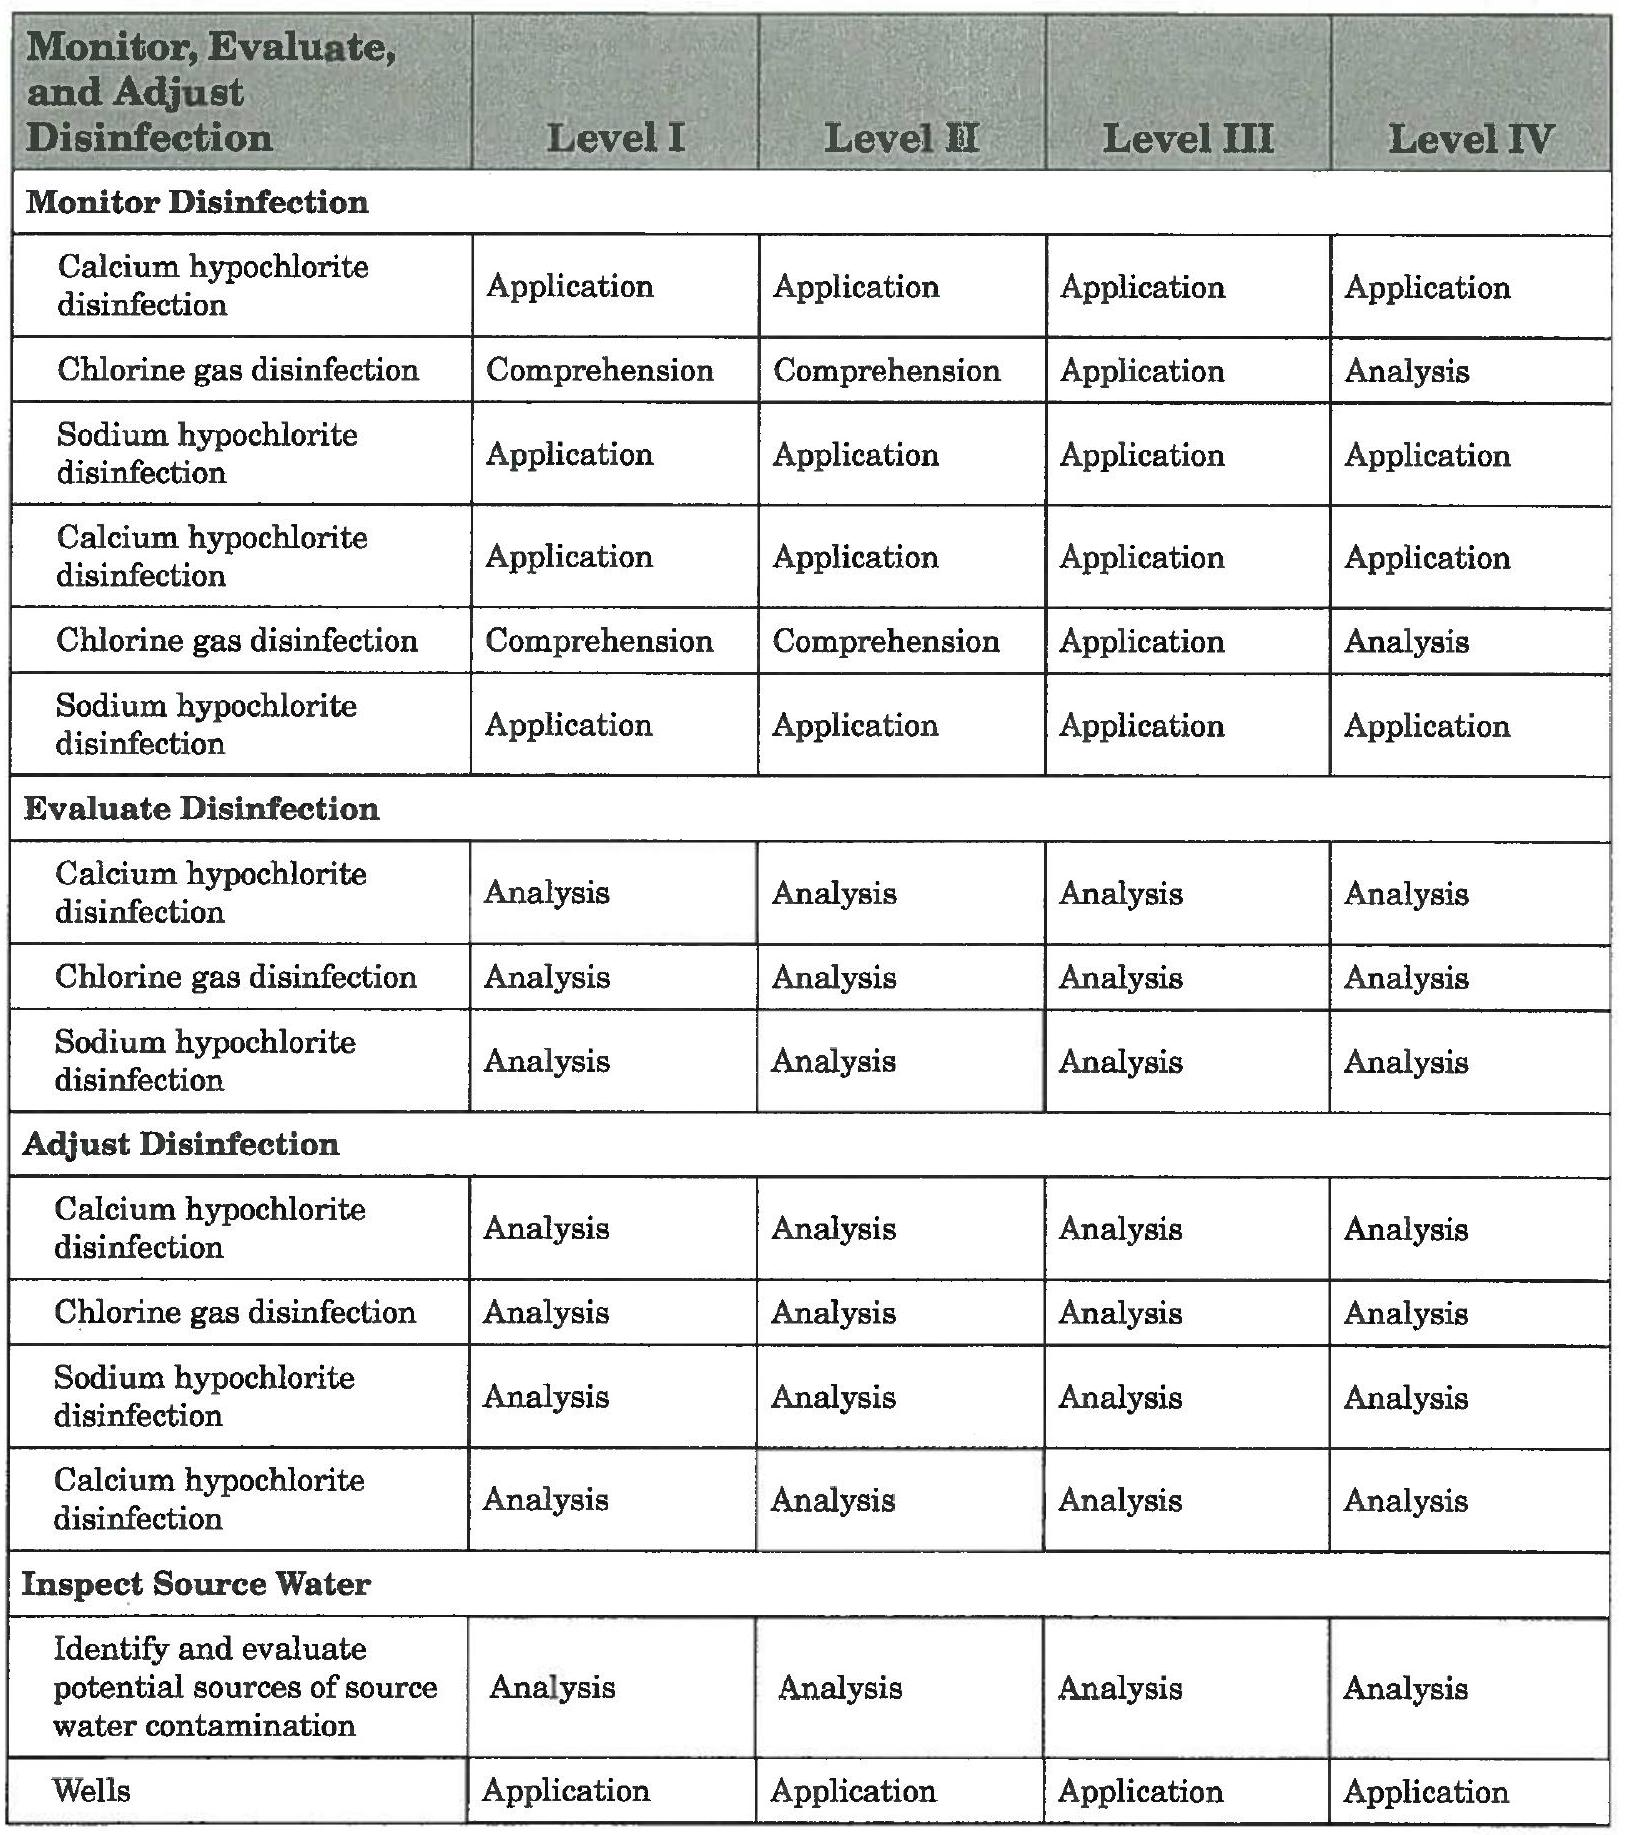
\includegraphics[max width=\textwidth]{2022_11_10_beeca89b60229885003dg-09}

\section{Required Capabillties}
\section{Knowledge of:}
\begin{itemize}
  \item Proper chemical handling and storing

  \item Regulations

  \item Reporting requirements

  \item Safe Drinking Water Act (SDWA)

  \item Safety procedures

  \item Sampling requirements

  \item Testing instruments

  \item Watershed management

  \item 40 CFR 141 Subpart C: Monitoring and Analytical Requirements (turbidity, coliforms, organic contaminants, organic contaminants)

  \item 40 CFR 141 Subpart D: Reporting and Recordkeeping Requirements

  \item 40 CFR 141 Subpart F: Maximum Contaminant Level Goals and Maximum Residual Disinfectant Level Goals

  \item 40 CFR 141 Subpart G: National Primary Drinking Water Regulations:

\end{itemize}

\section{Ability to:}
\begin{itemize}
  \item Adjust equipment

  \item Adjust flow patterns

  \item Adjust system units

  \item Calibrate equipment

  \item Calibrate instruments Maximum Contaminant Levels and Maximum Residual Disinfectant Lee

  \item 40 CFR 141 Subpart H: Filtration a Disinfection

  \item 40 CFR 141 Subpart L: Disinfectantum Residuals, Disinfection Byproducts, and Disinfection Byproduct Precurs:

  \item 40 CFR 141 Subpart P: Enhanced Filtration and Disinfection Systems . Serving 10,000 or More People

  \item 40 CFR 141 Subpart T: Enhanced Filtration and Disinfection Systems = Serving Fewer Than 10,000 People

  \item 40 CFR 141 Subpart U: Initial Distribution System Evaluations

  \item 40 CFR 141 Subpart V: Stage 2 Disinfection Byproducts Requireme $=$

\end{itemize}

\section{Monitor, Evaluate, and Adjust Disinfection}
\begin{itemize}
  \item Interpret data

  \item Perform distribution math

  \item Recognize normal and abnormal analytical results

\end{itemize}

\section{Sample Questions for Level I}
\section{Answers on page 341}
\begin{enumerate}
  \item One of chlorine's advantages is that it\\
a. is not influenced much by $\mathrm{pH}$ changes.\\
b. does not produce chlorinated by-products.\\
c. has a persistent residual.\\
d. does not cause taste and odor problems.

  \item Chlorine gas is times heavier than air.\\
a. $\quad 1.5$\\
b. $\quad 2.5$\\
c. $\quad 3.5$\\
d. $4.5$ 3. After a water storage tank has been chlorinated, which bacteriological test must prove negative before the tank is put back into service?\\
a. Gram negative test\\
b. HPC test\\
c. Coliform test\\
d. Chloramine test

  \item Which is the best and most reliable method for finding a very small chlorine leak?\\
a. Use soap on possible areas of leak and watch for bubbles\\
b. Use a strong ammonia solution on a cloth swab and place it by the suspected leak\\
c. Use methane gas and watch for a dark brown smoke\\
d. Use a chlorine gas detector and place it next to any area suspected of leaking

  \item The minimum required free chlorine residual anywhere in the distribution system is\\
a. a detectable level.\\
b. $\quad 0.2 \mathrm{mg} / \mathrm{L}$.\\
c. $0.4 \mathrm{mg} / \mathrm{L}$.\\
d. $0.5 \mathrm{mg} / \mathrm{L}$.

\end{enumerate}

\section{Sample Questions for Level II}
\section{Answers on page 341}
\begin{enumerate}
  \item Sodium hypochlorite $(\mathrm{NaOCl})$ solution is available with available chlorine.\\
a. 2 to $5 \%$\\
b. 5 to $20 \%$\\
c. 25 to $50 \%$\\
d. 50 to $70 \%$

  \item Booster chlorination is chlorine added\\
a. in the coagulation mixing chamber.\\
b. before the filters.\\
c. at the clearwell.\\
d. somewhere in the distribution system.

  \item According to AWWA Standard C651, disinfection of water mains requires 24-hour exposure to which minimum free chlorine residual?\\
a. $10 \mathrm{mg} / \mathrm{L}$\\
b. $25 \mathrm{mg} / \mathrm{L}$\\
c. $50 \mathrm{mg} / \mathrm{L}$\\
d. $100 \mathrm{mg} / \mathrm{L}$

  \item Which must be measured at least at the same time and at the same sampling points in the distribution system that total coliforms are sampled for a water system that only uses surface water?\\
a. $\mathrm{pH}$\\
b. Langelier Index\\
c. Residual disinfectant concentration\\
d. Heterotrophic bacteria 5. Hypochlorous acid is\\
a. a weak acid.\\
b. a strong acid.\\
c. easily dissociatable.\\
d. hydrophobic.

\end{enumerate}

\section{Sample Questions for Level III}
\section{Answers on page 341}
\begin{enumerate}
  \item Which chemical oxidant would be most effective for controlling biological growth?\\
a. Chloramines\\
b. Chlorine\\
c. Ozone\\
d. Potassium permanganate

  \item Which is the Maximum Residual Disinfectant Level for chlorine?\\
a. $\quad 4.0 \mathrm{mg} / \mathrm{L}$\\
b. $\quad 4.5 \mathrm{mg} / \mathrm{L}$\\
c. $\quad 5.0 \mathrm{mg} / \mathrm{L}$\\
d. $\quad 6.0 \mathrm{mg} / \mathrm{L}$

  \item Which is the most common hypochlorinator problem?\\
a. Clogged equipment\\
b. Cracked pump head\\
c. Corrosion\\
d. Broken plunger

  \item Which reaction will take longer with chlorine?\\
a. Hydrogen sulfide\\
b. Ammonia\\
c. Organic material\\
d. Calcium sulfide

  \item If the continuous monitoring of the residual disinfectant concentration for water entering the distribution system fails, how often must grab samples be collected in lieu of continuous monitoring until the problem is repaired?\\
a. Every hour\\
b. Every 4 hours\\
c. Every 8 hours\\
d. Every 12 hours

\end{enumerate}

\section{Sample Questions for Level IV}
\section{Answers on page 342}
\begin{enumerate}
  \item Which organisms have the greatest resistance to chlorine?\\
a. Viruses\\
b. Bacteria\\
c. Nematodes\\
d. Giardia cysts

  \item Which is the maximum residual for chlorine dioxide to avoid taste and odor complaints?\\
a. $0.4$ to $0.5 \mathrm{mg} / \mathrm{L}$\\
b. $0.9$ to $1.0 \mathrm{mg} / \mathrm{L}$\\
c. $1.3$ to $1.5 \mathrm{mg} / \mathrm{L}$\\
d. $1.9$ to $2.0 \mathrm{mg} / \mathrm{L}$

  \item If secondary chlorine is added to a distribution system that uses chloramines, the chlorine may be added to a desired chlorine to ammonia-nitrogen ratio of\\
a. $3.0: 1$ to $3.5: 1$\\
b. $3.5: 1$ to $4.0: 1$\\
c. $4.0: 1$ to $4.5: 1$\\
d. $4.5: 1$ to $5.0: 1$

  \item Gaseous chlorine dioxide is generated from\\
a. oxygen + chlorine gas $+$ heat (energy).\\
b. aqueous chlorine $+$ oxygen $+$ heat (energy).\\
c. sodium chlorite $+$ chlorine at low $\mathrm{pH}$ values.\\
d. hypochlorous acid $+$ oxygen $+$ organic catalyst.

  \item Which is the most probable solution if sulfur bacteria are causing corrosion in the distribution system?\\
a. Minimize pump activity\\
b. Acidification and cleaning\\
c. Optimize coagulation, flocculation, and filtration\\
d. Routine use of disinfectant and penetrant

\end{enumerate}

\section{Laboratory Analysis}
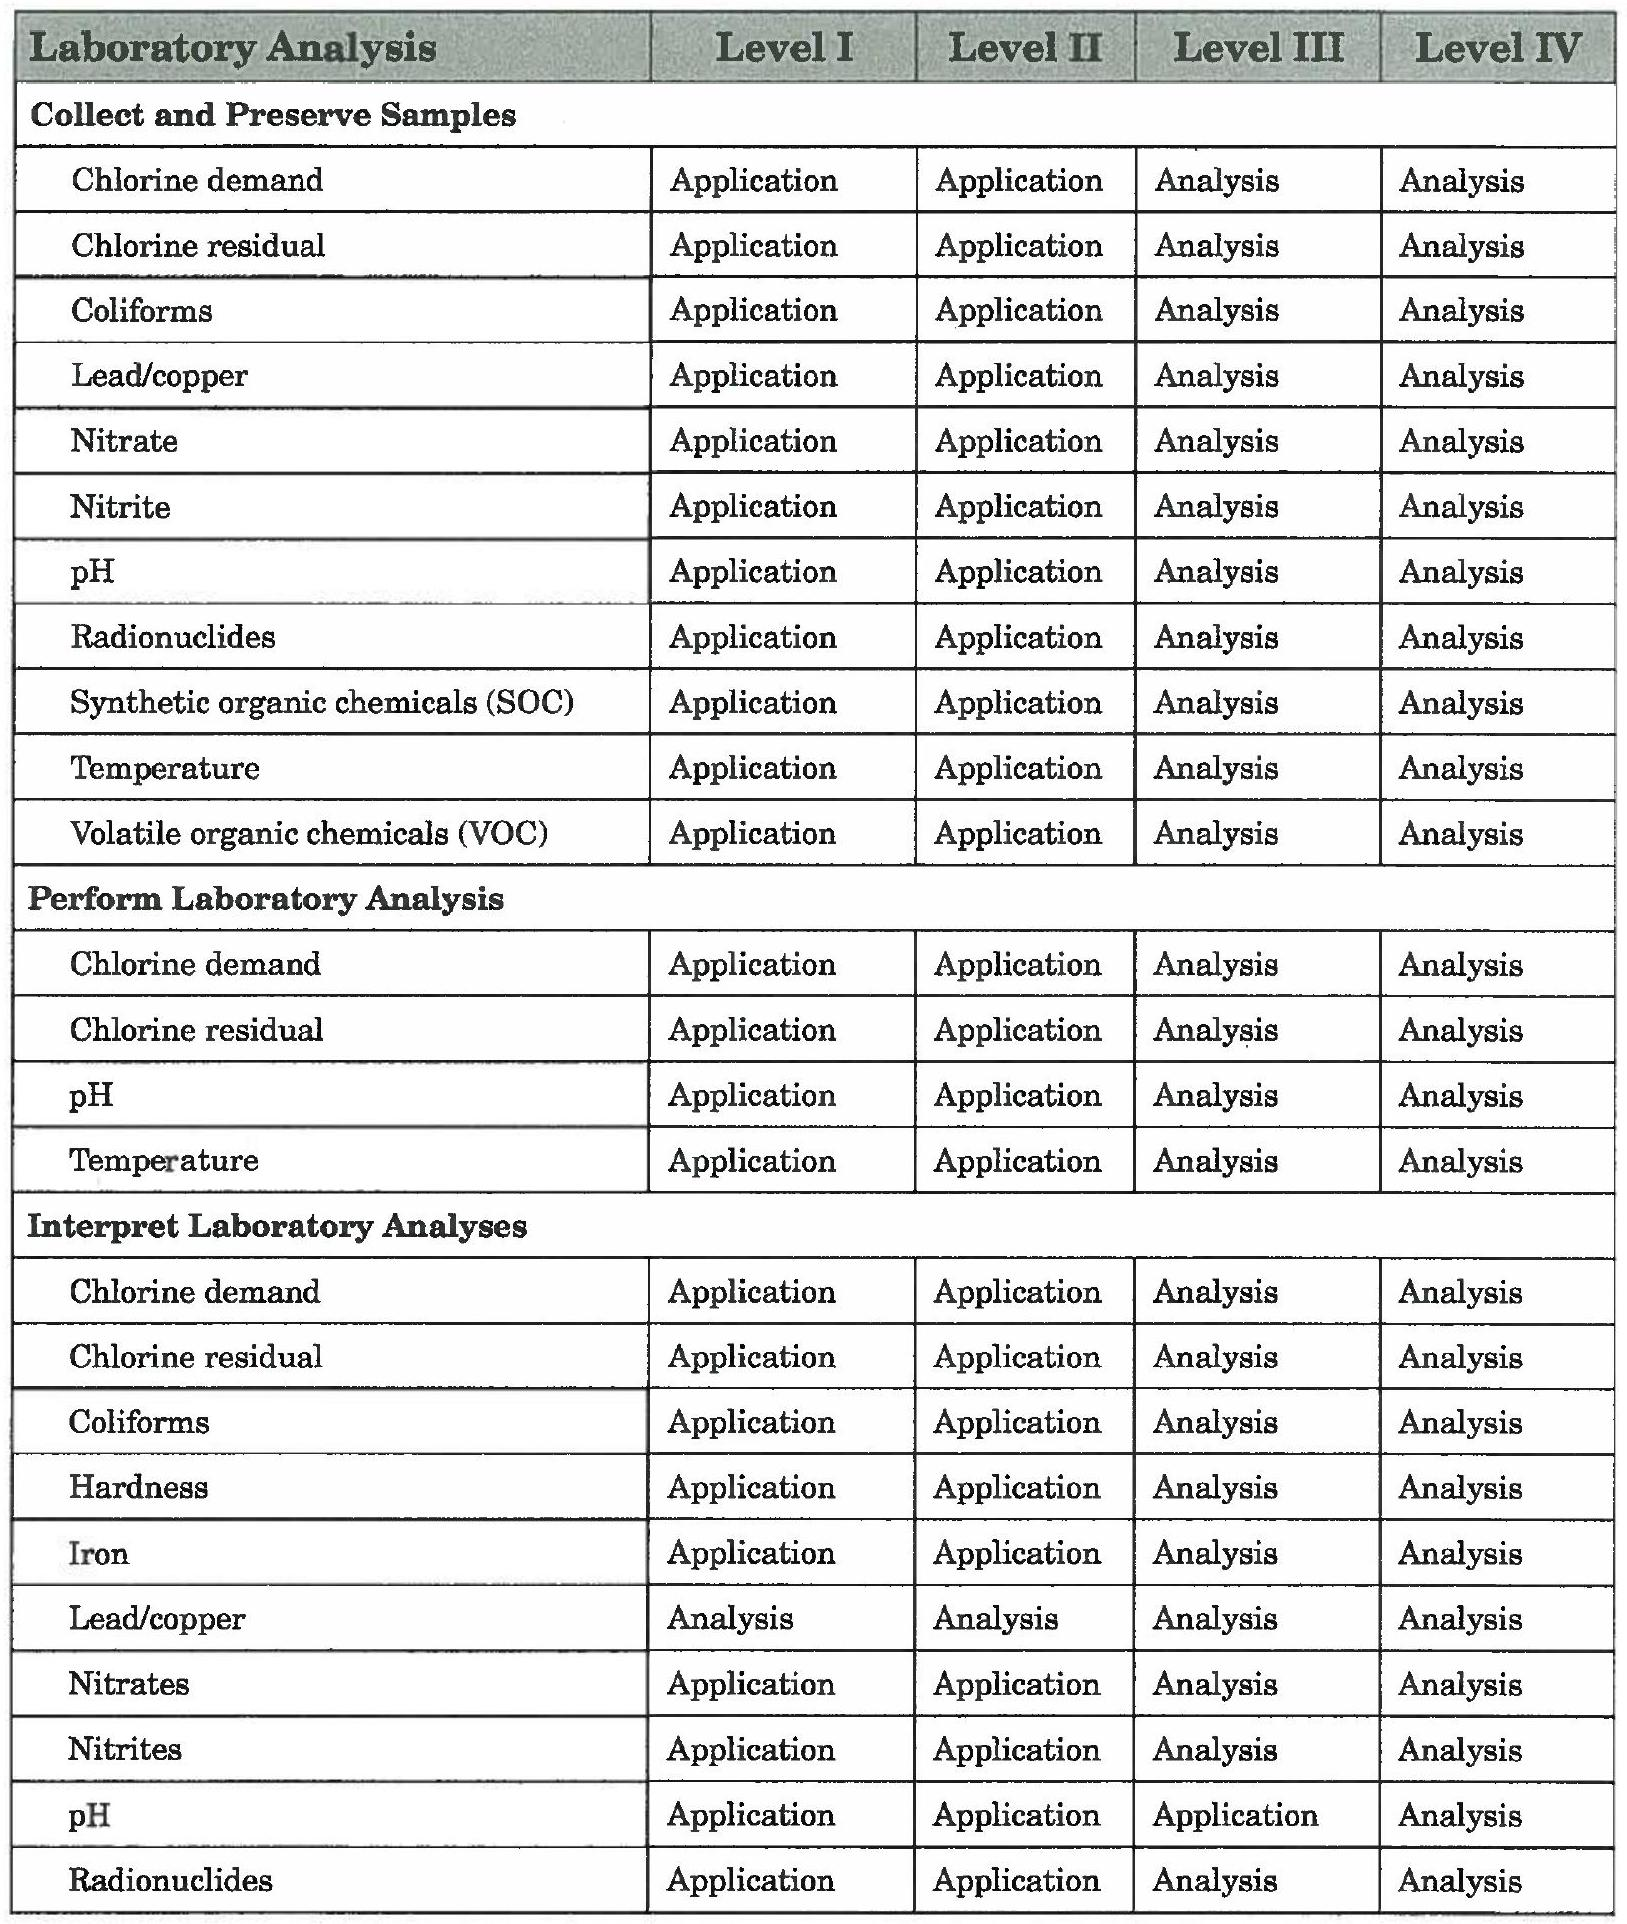
\includegraphics[max width=\textwidth]{2022_11_10_beeca89b60229885003dg-15}

\begin{tabular}{|l|l|l|l|l|}
\hline
Synthetic organic chemicals (SOC) & Application & Application & Analysis & Analysis \\
\hline
Temperature & Application & Application & Application & Analysis \\
\hline
Turbidity & Application & Application & Application & Analysis \\
\hline
Volatile organic chemicals (VOC) & Application & Application & Analysis & Analysis \\
\hline
\end{tabular}

\section{Required Capabilities}
\section{Knowledge of:}
\begin{itemize}
  \item Biological science

  \item Disinfection concepts

  \item Disinfection design parameters

  \item Disinfection process

  \item General chemistry

  \item Laboratory equipment

  \item Monitoring requirements

  \item Normal characteristics of water

  \item Physical science

  \item Proper chemical handling and storing

  \item Proper sampling procedures

  \item Quality control/quality assurance practices

  \item Record keeping policies

  \item Regulations

  \item Reporting requirements

  \item Safe Drinking Water Act (SDWA)

  \item Safety procedures

  \item Sampling requirements

  \item Testing instruments

  \item 40 CFR 141 Subpart B: Maximum Contaminant Levels (arsenic, nitrate, turbidity)

  \item 40 CFR 141 Subpart C: Monitoring and Analytical Requirements (turbidity, coliforms, organic contaminants, organic contaminants)

\end{itemize}

\section{Ability to:}
\begin{itemize}
  \item Calibrate equipment

  \item Calibrate instruments

  \item Determine what information needs to be recorded

  \item Diagnose/troubleshoot equipment

  \item Follow written procedures

  \item Interpret data

  \item Interpret Material Safety Data Sheets - 40 CFR 141 Subpart D: Reporting and Recordkeeping Requirements

  \item 40 CFR 141 Subpart E: Special Regulations, Including Monitoring Regulations and Prohibition on Lead Use

  \item 40 CFR 141 Subpart F: Maximum Contaminant Level Goals and Maximum Residual Disinfectant Level Goals

  \item 40 CFR 141 Subpart G: National Primary Drinking Water Regulations: Maximum Contaminant Levels and Maximum Residual Disinfectant Levels

  \item 40 CFR 141 Subpart H: Filtration and Disinfection

  \item 40 CFR 141 Subpart I: Control of Lead and Copper

  \item 40 CFR 141 Subpart L: Disinfectant Residuals, Disinfection By-products, and Disinfection By-product Precursors

  \item 40 CFR 141 Subpart S: Ground Water Rule

  \item 40 CFR 141 Subpart V: Stage 2 Disinfection By-products Requirements - Organize information

  \item Recognize normal and abnormal analytical results

  \item Record information

  \item Review reports

  \item Transcribe data

  \item Translate technical language into common terminology

\end{itemize}

\section{Laboratory Analysis}
\section{Sample Questions for Level I}
\section{Answers on page 343}
\begin{enumerate}
  \item First draw samples for the analysis of lead and copper water must be collected from taps where the water has stood motionless in the plumbing for at least\\
a. 4 hours.\\
b. 6 hours.\\
c. 8 hours.\\
d. 24 hours.

  \item Samples to be tested for coliforms are collected in plastic bottles that must contain\\
a. sodium thiocarbonate.\\
b. sodium thiooxalate.\\
c. sodium thiosulfate.\\
d. sodium thiocyanate.

  \item The volume of a sample for coliform compliance is\\
a. $100 \mathrm{~mL}$.\\
b. $200 \mathrm{~mL}$.\\
c. $300 \mathrm{~mL}$.\\
d. 0 ; there is no volume compliance for coliforms.

  \item If a water sample is not analyzed immediately for chlorine residual, it is acceptable if it is analyzed within\\
a. 10 minutes.\\
b. 15 minutes.\\
c. 20 minutes.\\
d. 30 minutes.

  \item Which may be substituted for the analysis of residual disinfectant concentration, when total coliforms are also sampled at the same sampling point?\\
a. Heterotrophic plate count (HPC)\\
b. Fecal coliforms\\
c. Giardia lamblia\\
d. Combined chlorine

\end{enumerate}

\section{Sample Questlons for Level II}
\section{Answers on page 343}
\begin{enumerate}
  \item Which water quality parameter requires a grab sample because it cannot be collected as a composite sample?\\
a. $\mathrm{pH}$\\
b. Iron\\
c. Nitrate\\
d. Zinc 2. One chemical characteristic of an acid is that it will\\
a. accept an electron pair.\\
b. donate an electron pair.\\
c. accept a proton.\\
d. accept a neutron.

  \item Which chemical contains calcium?\\
a. Soda ash\\
b. Lime\\
c. Caustic soda\\
d. Sodium bicarbonate

  \item The best choice to collect a water sample from a customer's faucet in regards to a complaint would be a\\
a. faucet without threads.\\
b. faucet that can swivel.\\
c. single-lever handle faucet.\\
d. faucet with an aerator.

  \item When measuring for free chlorine residual, which method is the quickest and simplest?\\
a. DPD color comparater\\
b. Orthotolidine method\\
c. Amperometric titration\\
d. 1, 2 nitrotoluene di-amine method

\end{enumerate}

\section{Sample Questions for Level III}
\section{Answers on page 343}
\begin{enumerate}
  \item Water that is to be analyzed for inorganic metals should be acidified with\\
a. dilute hydrochloric acid.\\
b. concentrated hydrochloric acid.\\
c. dilute nitric acid.\\
d. concentrated nitric acid.

  \item If a public water system does not continuously monitor turbidity, how often must it collect a grab sample to measure turbidity from the system's filtered water?\\
a. Every 2 hours\\
b. Every 4 hours\\
c. Every 8 hours\\
d. Every 12 hours

  \item If a water system uses chlorine for disinfection, but does not provide filtration, which daily parameters following each point of disinfection are required for determining CT calculations?\\
a. Lowest value for chlorine residual, pH and temperature, and highest alkalinity\\
b. Lowest value for chlorine residual and contact time, lowest temperature, and highest $\mathrm{pH}$\\
c. Lowest value for chlorine residual, lowest $\mathrm{pH}$, and lowest temperature\\
d. Lowest value for chlorine residual and contact time, $\mathrm{pH}$ and alkalinity, and highest temperature 4. A water system exceeds the lead action level if the concentration in more than $10 \%$ of tap water samples collected during any monitoring period conducted is greater than\\
a. $0.010 \mathrm{mg} / \mathrm{L}$.\\
b. $0.012 \mathrm{mg} / \mathrm{L}$.\\
c. $0.015 \mathrm{mg} / \mathrm{L}$.\\
d. $0.020 \mathrm{mg} / \mathrm{L}$.

  \item A water system can reduce its monitoring of total organic carbon (TOC), if it achieves which of the following?\\
a. TOC $<1.0 \mathrm{mg} / \mathrm{L}$ for 1 year or $<0.5 \mathrm{mg} / \mathrm{L}$ for $6 \mathrm{months}$\\
b. TOC $<2.0 \mathrm{mg} / \mathrm{L}$ for 1 year or $<1.0 \mathrm{mg} / \mathrm{L}$ for $6 \mathrm{months}$\\
c. TOC $<2.0 \mathrm{mg} / \mathrm{L}$ for 2 years or $<1.0 \mathrm{mg} / \mathrm{L}$ for 1 year\\
d. TOC $<3.0 \mathrm{mg} / \mathrm{L}$ for 2 years or $<2.0 \mathrm{mg} / \mathrm{L}$ for 1 year

\end{enumerate}

\section{Sample Questions for Level IV}
\section{Answers on page 344}
\begin{enumerate}
  \item Under the Lead and Copper Rule of the Safe Drinking Water Act, how is the 90th percentile of lead determined for a water system serving fewer than 100 people if the system collects only 5 samples per monitoring period?\\
a. By taking the average of the highest and second highest concentrations\\
b. By allowing the sample result with the highest concentration to be the 90 th percentile value\\
c. By allowing the system 2 monitoring periods before reporting\\
d. By multiplying the two highest values by $0.9$, then taking the average of this result

  \item A surface water system can reduce the number of samples for total trihalomethanes (TTHM) and the sum of five haloacetic acids (HAA5), if it has monitored for at least one year and\\
a. TTHM $\leq 0.020 \mathrm{mg} / \mathrm{L}$ and HAA5 $\leq 0.010 \mathrm{mg} / \mathrm{L}$.\\
b. TTHM $\leq 0.030 \mathrm{mg} / \mathrm{L}$ and HAA5 $\leq 0.020 \mathrm{mg} / \mathrm{L}$.\\
c. TTHM $\leq 0.040 \mathrm{mg} / \mathrm{L}$ and HAA5 $\leq 0.030 \mathrm{mg} / \mathrm{L}$.\\
d. TTHM $\leq 0.060 \mathrm{mg} / \mathrm{L}$ and HAA5 $\leq 0.040 \mathrm{mg} / \mathrm{L}$.

  \item A water system that uses chlorine dioxide may reduce the sampling frequency in the distribution system from one three-sample set per month to after one year of monitoring where no individual chlorite sample collected in the distribution system exceeded the chlorite MCL.\\
a. one three-sample set per quarter\\
b. one six-sample set semi-annually\\
c. one three-sample set annually\\
d. one six-sample set annually 4. If a water system collects at least 40 samples per month for the analyses of total coliforms, which percent of total coliform positive samples are acceptable for the system to remain in compliance with the maximum contaminant level for total coliforms?\\
a. No more than $2 \%$\\
b. No more than $3 \%$\\
c. No more than $4 \%$\\
d. No more than $5 \%$

  \item If a water system changes its disinfection sampling point, disinfection type, process, or any other modification identified by the state, it must\\
a. perform a sanitary survey.\\
b. develop a disinfection benchmark.\\
c. develop a disinfection profile.\\
d. start over or go back to routine monitoring of disinfection by-products.

\end{enumerate}

\section{Install Equipment}
\begin{tabular}{|l|l|l|l|l|}
\hline
Install Equipment & \multicolumn{1}{|c|}{Level I} & \multicolumn{1}{c|}{Level II} & \multicolumn{1}{c|}{Level III} & \multicolumn{1}{c|}{Level IV} \\
\hline
Backflow prevention devices & Comprehension & Comprehension & Comprehension & Comprehension \\
\hline
Hydrants & Comprehension & Application & Application & Application \\
\hline
Meters & Application & Application & Application & Application \\
\hline
Piping & Comprehension & Application & Application & Application \\
\hline
Service connections & Comprehension & Application & Application & Application \\
\hline
Taps & Comprehension & Application & Application & Analysis \\
\hline
Valves & Comprehension & Application & Application & Analysis \\
\hline
Water mains & Comprehension & Application & Application & Analysis \\
\hline
\end{tabular}

\section{Required Capabilities}
\section{Knowledge of:}
\begin{itemize}
  \item Approved backflow methods and devices

  \item Blueprint readings

  \item Building codes

  \item Corrosion control process (including cathodic protection)

  \item Dechlorination process

  \item Different types of cross-connections

  \item Different types of joints, restraints, and thrust blocks

\end{itemize}

\section{Ability to:}
\begin{itemize}
  \item Demonstrate safe work habits

  \item Diagnose/troubleshoot equipment

  \item Identify potential safety hazards

  \item Inspect pumps

  \item Operate safety equipment - Function of tools

  \item Personal protective equipment

  \item Pipe fittings and joining methods

  \item Piping material, type, and size

  \item Pneumatics

  \item Proper lifting techniques

  \item Protective coatings and paints

  \item Safety procedures - Perform distribution math

  \item Recognize unsafe work conditions

  \item Select safety equipment

  \item Use hand tools

  \item Use power tools

\end{itemize}

\section{Install Equipment}
\section{Sample Questions for Level I}
\section{Answers on page 345}
\begin{enumerate}
  \item It is standard practice to install fire hydrants on mains that are at a minimum or larger.\\
a. 6 inches\\
b. 8 inches\\
c. 10 inches\\
d. 12 inches

  \item A corporation stop is used for a\\
a. service line.\\
b. pump discharge line.\\
c. tank inlet.\\
d. tank outlet.

  \item When PVC pipe is stacked loose, it should not be stacked more than how high?\\
a. $2.0$ feet\\
b. $3.0$ feet\\
c. $5.0$ feet\\
d. $7.5$ feet

  \item Which is the most common cause for pipe joint failure (leaking) in newly laid pipe\\
a. The use of a cracked gasket\\
b. Not pushing the spigot end the full distance into the bell\\
c. Not having the joint completely clean\\
d. An incorrect trench bedding angle

  \item Which should be installed at a dead-end water main?\\
a. Vacuum valve\\
b. Air valve\\
c. Blowoff valve\\
d. Water quality sampling station

\end{enumerate}

\section{Sample Questions for Level II}
\section{Answers on page 345}
\begin{enumerate}
  \item Compression fittings used with copper or plastic tubing seal by means of a\\
a. beveled sleeve.\\
b. compression ring.\\
c. compressed beveled gasket.\\
d. compressed o-rings located at either end of the fitting's beveled neck. 2. The breaking of a buried pipe when it is unevenly supported is called\\
a. stress breakage.\\
b. shear breakage.\\
c. beam breakage.\\
d. flexural breakage.

  \item Thrust from a water surge almost always acts pushes against. to the inside surface that it\\
a. vertically\\
b. horizontally\\
c. perpendicular\\
d. vertically and horizontally

  \item Which thrust control is easy to use, especially in locations where existing utilities or structures are numerous?\\
a. Restraining fittings\\
b. Tie rods\\
c. Thrust anchors\\
d. Thrust blocks

  \item The backfill material for a pipe installation should contain enough to allow for thorough compaction.\\
a. moisture\\
b. sand\\
c. gravel\\
d. mixed sizes

\end{enumerate}

\section{Sample Questions for Level III}
\section{Answers on page 345}
\begin{enumerate}
  \item A bypass valve would be used with a\\
a. gate valve.\\
b. butterfly valve.\\
c. needle valve.\\
d. diaphragm valve.

  \item Where ground frost is expected, the riser pipes in a meter pit should be at least how far away from any wall of the meter box to prevent freezing?\\
a. 1 to 2 inches\\
b. 2 to 4 inches\\
c. 4 to 6 inches\\
d. 6 to 8 inches 3. How can a distribution operator tell if a new pipe with no obvious cracks or chips is good before it is placed in the trench for installation?\\
a. By conducting a pressure test\\
b. By gently tapping the length of the pipe with a hammer; the pipe should ring or hum clearly\\
c. By attaching a sonic meter at one end and listening at other end with headphones; any defects will give crackling sounds\\
d. By placing a sonic meter at one end and an oscilloscope at the other end; defects will show up as sharp peaks and valleys as pitch is varied; no defects if only have smooth curves as pitch is varied

  \item Which is the recommended trench width for a 42-inch diameter ductile-iron pipe?\\
a. 58 inches\\
b. 60 inches\\
c. 66 inches\\
d. 72 inches

  \item The first layer of backfill if compaction is required for a newly installed pipe should come up to\\
a. the bottom of the pipe.\\
b. one-third up the bottom of the pipe.\\
c. the centerline of the pipe.\\
d. the top of the pipe.

\end{enumerate}

\section{Sample Questions for Level IV}
\section{Answers on page 346}
\begin{enumerate}
  \item If special bedding material is required by the design engineer due to poor local soil conditions, the material should not contain granular material greater than\\
a. $\frac{1}{4}$ inch.\\
b. $\frac{1}{2}$ inch.\\
c. $\frac{3}{4}$ inch.\\
d. 1 inch.

  \item How much will a flexible disk coupling compensate for in parallel misalignment?\\
a. $\frac{1}{32}$ inch\\
b. $\frac{1}{16}$ inch\\
c. $\frac{1}{8}$ inch\\
d. $\frac{1}{4}$ inch

  \item Which will a flexible diaphragm coupling compensate for in angular movement?\\
a. $1.0$ degree\\
b. $2.0$ degrees\\
c. $3.7$ degrees\\
d. $4.0$ degrees 4. When a pressure reducing and a pressure sustaining valve are used in combination, one valve can keep a constant pressure even with fluctuating demand, while the other valve holds the pressure at a minimum predetermined\\
a. upstream; flow\\
b. upstream; pressure\\
c. downstream; flow\\
d. downstream; pressure

  \item If backsiphonage occurs with a reduced-pressure device and the pressure drops below 2 psi, which process will occur?\\
a. A vacuum will occur between the check valves, closing the check valve on the customer's side and fully opening the relief valve\\
b. A vacuum will occur on the supply side closing both check valves and fully opening the relief valve\\
c. The customer's check valve will close due to atmospheric pressure between the check valves, causing the relief valve to fully open\\
d. The relief valve will remain fully open and an air gap (atmospheric pressure) will form between the check valves, closing them both

\end{enumerate}

\section{Operate Equipment}
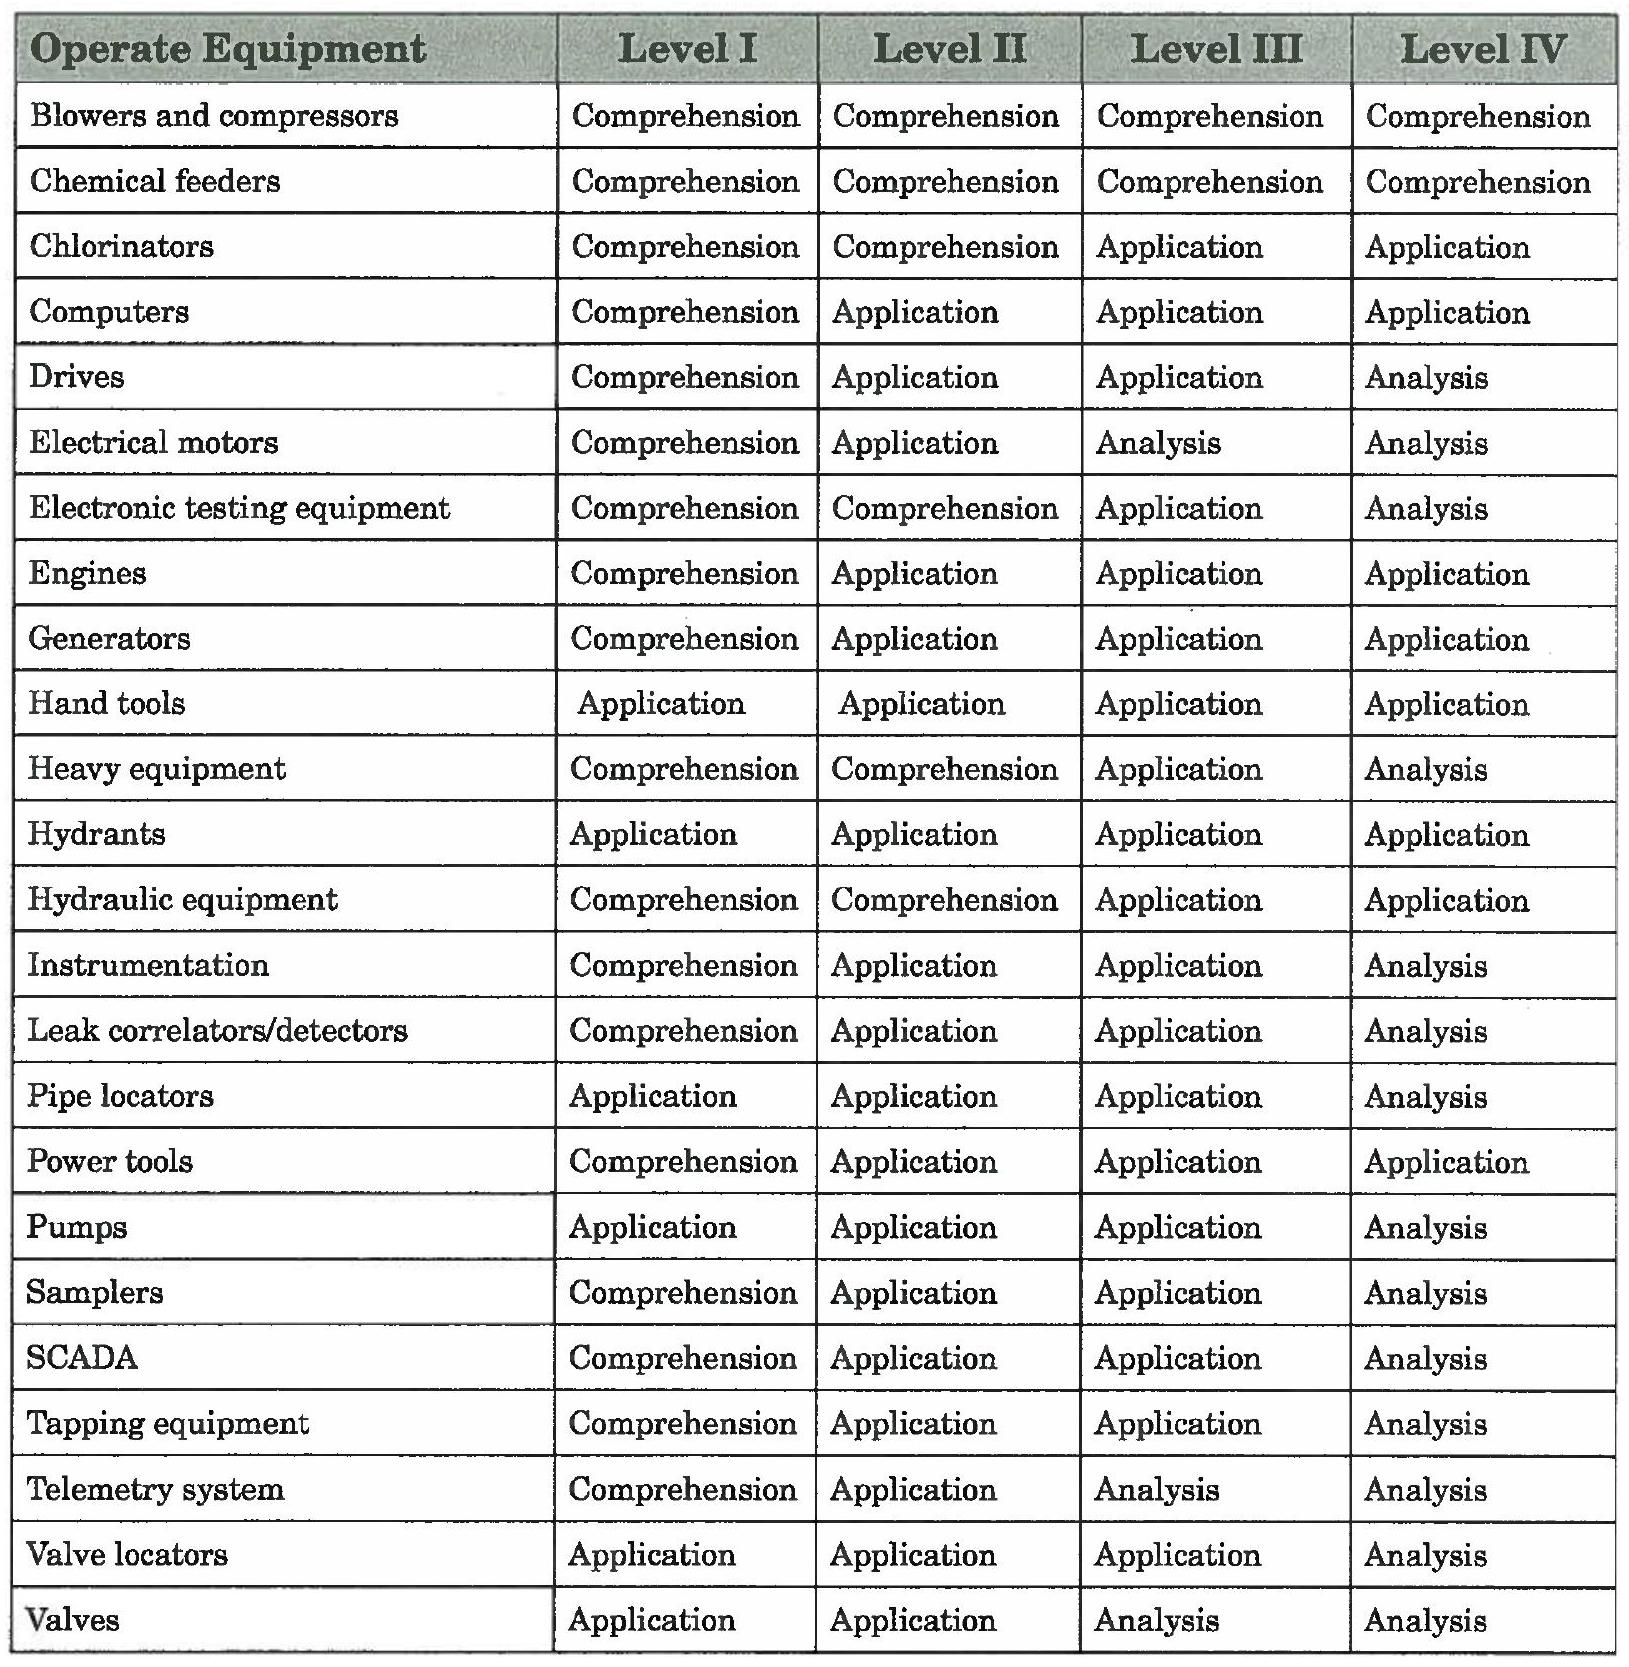
\includegraphics[max width=\textwidth]{2022_11_10_beeca89b60229885003dg-27}

\section{Required Capabillties}
\section{Knowledge of:}
\begin{itemize}
  \item Facility operation and maintenance

  \item Function of tools

  \item General electrical principles

  \item General hydraulic principles

  \item General mechanical principles

  \item Internal combustion engines

  \item Lubricant and fluid characteristics

  \item Operation and maintenance practices

\end{itemize}

\section{Abillty to:}
\begin{itemize}
  \item Adjust equipment

  \item Adjust flow patterns

  \item Adjust system units

  \item Calibrate equipment

  \item Calibrate instruments

  \item Demonstrate safe work habits

  \item Operate safety equipment - Pipe fittings and joining methods

  \item Piping material, type and size

  \item Pneumatics

  \item Quality control/quality assurance practices

  \item Start-up and shut down procedures

  \item Testing instruments

\end{itemize}

\section{Operate Equipment:}
\section{Sample Questions for Level I}
\section{Answers on page 347}
\begin{enumerate}
  \item The "heart" of a pump is called the\\
a. volute case.\\
b. impeller.\\
c. motor.\\
d. pump.
\end{enumerate}

\begin{itemize}
  \item Perform distribution math

  \item Perform physical measurements

  \item Recognize unsafe work conditions

  \item Select safety equipment

  \item Use hand tools

  \item Use power tools

\end{itemize}

\begin{enumerate}
  \setcounter{enumi}{1}
  \item Which device serves the same function as the packing?\\
a. Inline suction gland\\
b. Packing gland\\
c. Mechanical seal\\
d. Lantern seal

  \item Which is used to stop air leakage into the casing around a pump shaft?\\
a. Packing gland\\
b. Lantern ring\\
c. Seals\\
d. Shaft sleeves

  \item Which is at the top of a stuffing box?\\
a. Packing gland\\
b. Lantern ring\\
c. Mechanical seal\\
d. Seal cage 5. Which assembly holds the lantern ring and packing?\\
a. Shaft assembly\\
b. Casing ring assembly\\
c. Packing gland casing\\
d. Stuffing box

\end{enumerate}

\section{Sample Questions for Level II}
\section{Answers on page 347}
\begin{enumerate}
  \item Which of the following prevents the impeller of a pump from turning on the shaft?\\
a. Lock nut on threaded shaft\\
b. Key\\
c. Steel pin\\
d. Caliper pin

  \item Which type of valve is used to isolate a pump on the suction side?\\
a. Butterfly valve\\
b. Globe valve\\
c. Gate valve\\
d. Ball valve

  \item Water hammer can be described as\\
a. particle waves.\\
b. acoustic waves.\\
c. rogue waves.\\
d. longitudinal waves.

  \item When fully opened, which valve will have the highest head loss?\\
a. Gate valve\\
b. Plug valve\\
c. Globe valve\\
d. Ball valve

  \item Which type of pressure sensor uses a wire fastened to a diaphragm?\\
a. Bellows sensor\\
b. Strain gauge\\
c. Helical sensor\\
d. Diaphragm element

\end{enumerate}

\section{Sample Questions for Level III}
\section{Answers on page 348}
\begin{enumerate}
  \item Which two forces determine the behavior of electricity?\\
a. Static and dynamic forces\\
b. Dynamic and induced forces\\
c. Electric and magnetic forces\\
d. Amperage and voltage forces 2. The height a liquid can be raised vertically by a given pressure is called\\
a. pressure head.\\
b. total head.\\
c. velocity head.\\
d. pump head.

  \item A split case pump has three impellers. Which type of multistage pump is this?\\
a. One stage\\
b. Two stage\\
c. Three stage\\
d. Six stage

  \item A split case pump has two equal smaller impellers placed on either side of two equally sized large impellers. How many stages does this pump have?\\
a. One stage\\
b. Two stages\\
c. Four stages\\
d. Eight stages

  \item A pump loses its prime because the suction line has an air pocket. Which is the best solution?\\
a. Check pump's amperage and be sure pump's strainer is clean\\
b. Clean or repair priming unit\\
c. Open suction piping air bleed-off valves\\
d. Check external water seal unit

\end{enumerate}

\section{Sample Questions for Level IV}
\section{Answers on page 348}
\begin{enumerate}
  \item The lowest pressure point in the pump is the\\
a. center of the impeller.\\
b. outermost part of the impeller.\\
c. suction side of the pump.\\
d. discharge side of the pump.

  \item The shaft's main function is to transmit from the motor to the impeller.\\
a. centrifugal force\\
b. torque\\
c. kinetic energy\\
d. thrust

  \item Which is the range of specific speeds for a propeller pump?\\
a. 500 to $5,000 \mathrm{rpm}$\\
b. 5,000 to $9,000 \mathrm{rpm}$\\
c. 9,000 to $15,000 \mathrm{rpm}$\\
d. 12,000 to $18,000 \mathrm{rpm}$ 4. A vertical turbine pump would most likely have a specific speed of\\
a. 3,000 rpm.\\
b. $\quad 6,000$ rpm.\\
c. $9,000 \mathrm{rpm}$.\\
d. $12,000 \mathrm{rpm}$.

  \item Which is the most common cause for surges in the distribution system?\\
a. Power failure shutting down a pump suddenly\\
b. Valve opening and closing\\
c. Failure of flow on pressure regulation\\
d. Pump start-up

\end{enumerate}

\section{Perform Maintenance}
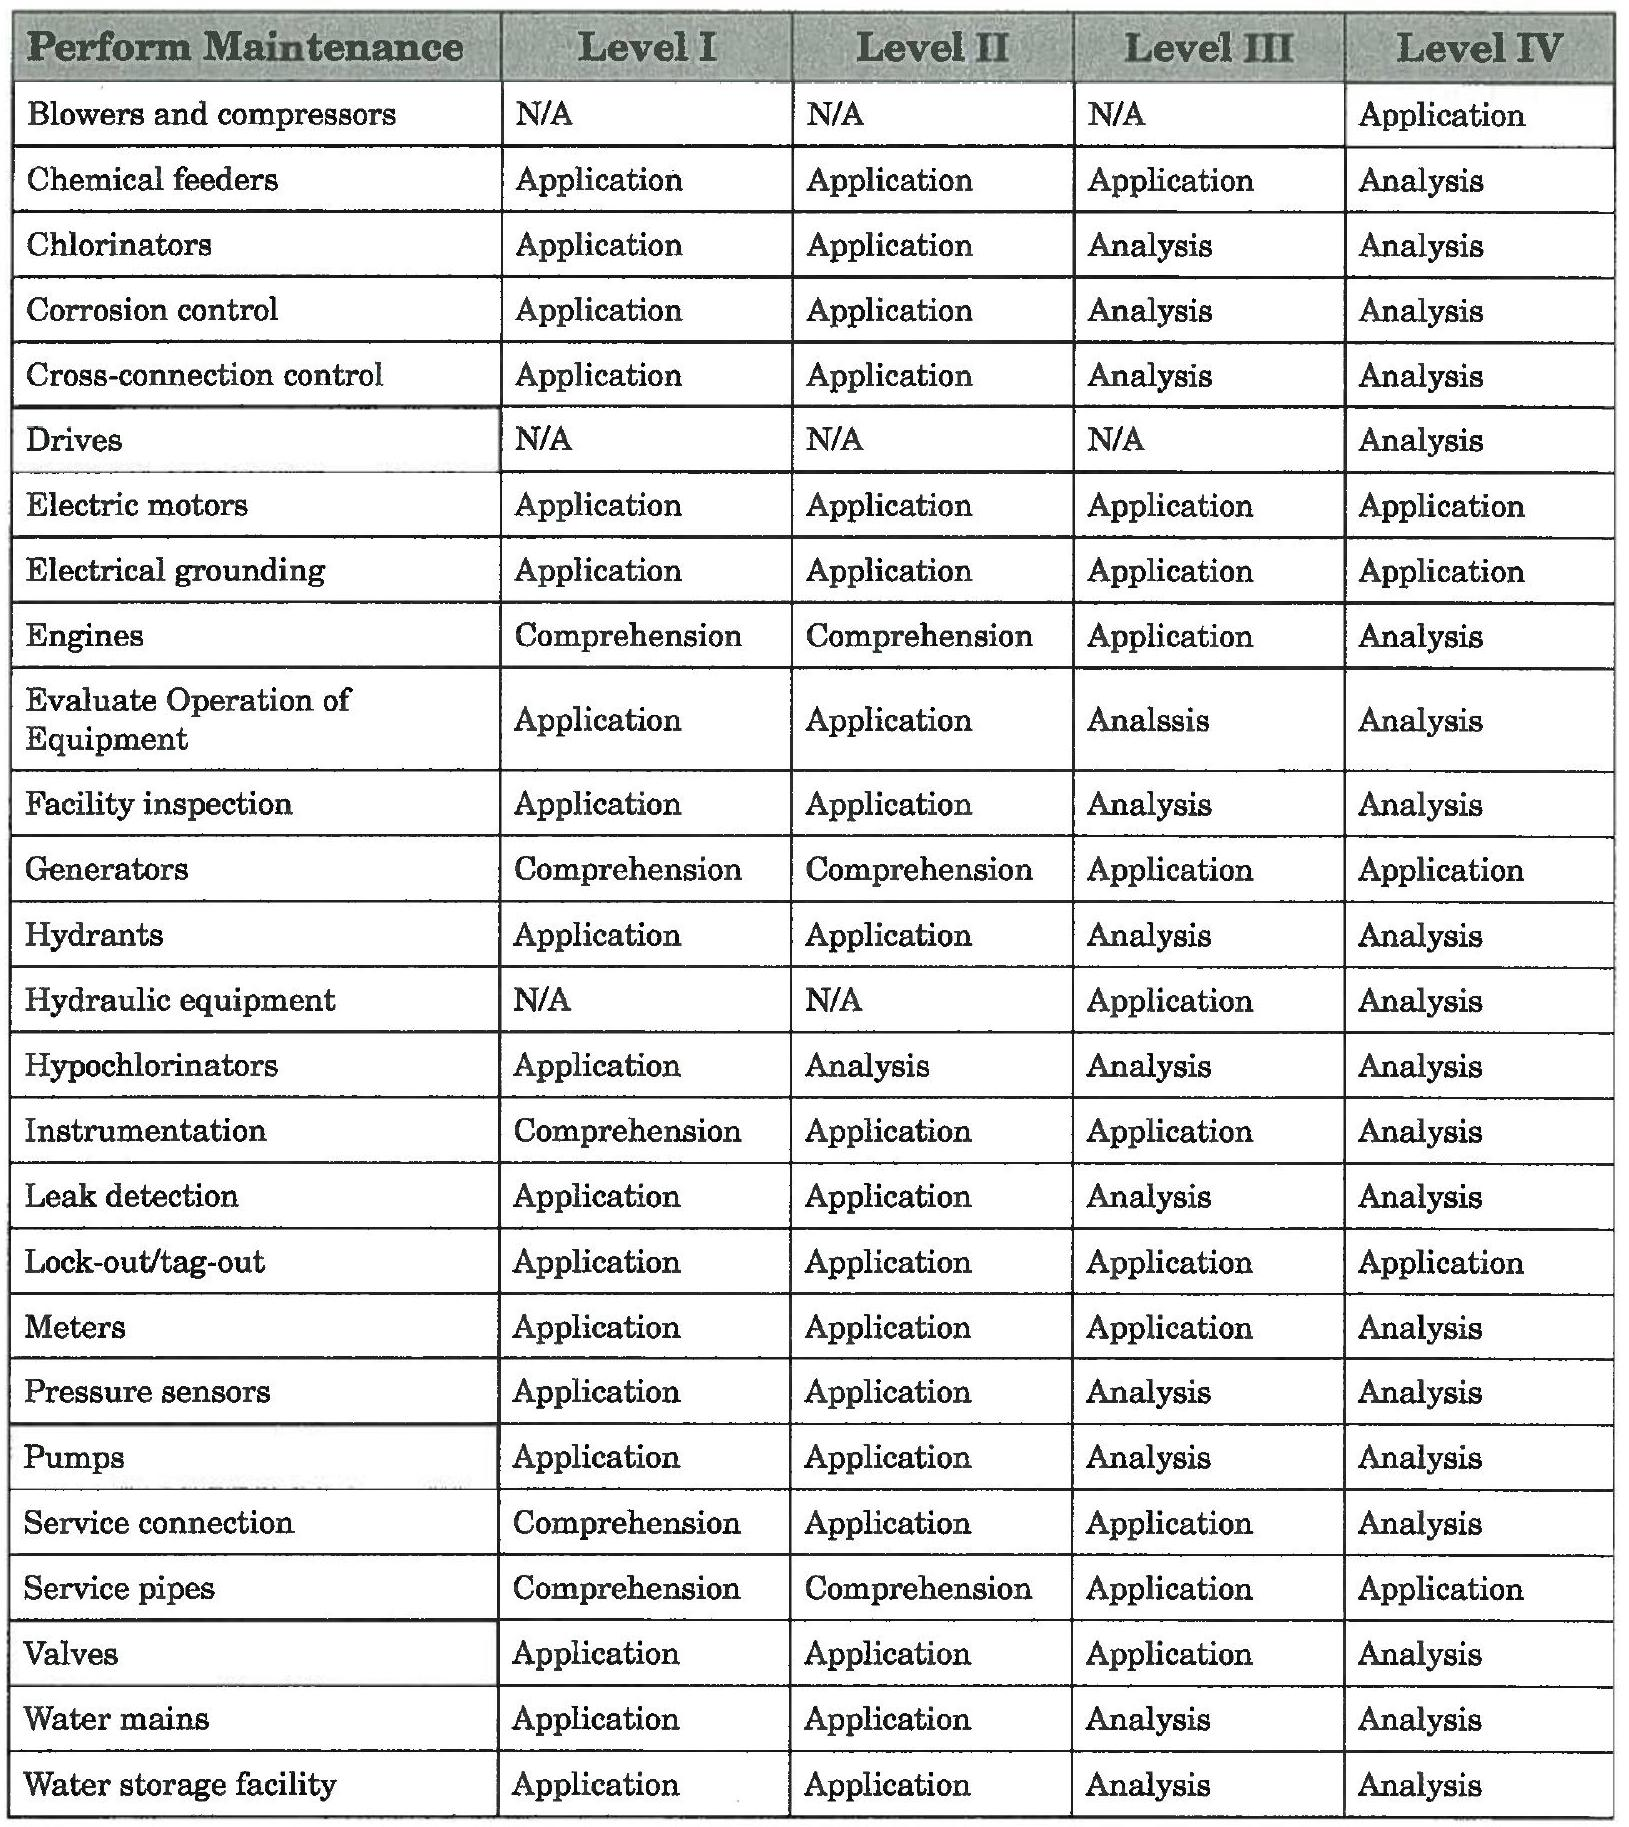
\includegraphics[max width=\textwidth]{2022_11_10_beeca89b60229885003dg-33}

\section{Required Capabillties}
\section{Knowledge of:}
\begin{itemize}
  \item Approved backflow methods and devices

  \item Blueprint readings

  \item Building codes

  \item Corrosion control process (including cathodic protection)

  \item Different types of cross-connections

  \item Different types of joints, restraints, and thrust blocks

  \item Facility operation and maintenance

  \item Facility security

  \item Function of tools

  \item General electrical principles

  \item General hydraulic principles

  \item General mechanical principles

  \item Internal combustion engines

  \item Laboratory equipment

  \item Local codes and ordinances

  \item Lubricant and fluid characteristics

\end{itemize}

\section{Abllity to:}
\begin{itemize}
  \item Adjust equipment

  \item Adjust flow patterns

  \item Adjust system units

  \item Assess likelihood of disaster occurring

  \item Assign work to proper trade

  \item Calibrate equipment

  \item Calibrate instruments

  \item Demonstrate safe work habits

  \item Diagnose/troubleshoot equipment

  \item Diagnose/troubleshoot system units

  \item Differentiate between preventative/ corrective maintenance

  \item Discriminate between normal/abnormal conditions

  \item Evaluate facility performance

  \item Evaluate operation of equipment

  \item Evaluate system units

  \item Identify potential safety hazards

  \item Inspect pumps

  \item Interpret data

  \item Interpret Material Safety Data Sheets

  \item Maintain inventory control system - Measuring instruments

  \item Operation and maintenance practices

  \item Personal protective equipment

  \item Pipe fittings and joining methods

  \item Piping material, type, and size

  \item Pneumatics

  \item Potential causes of disasters in facility

  \item Potential impact of disasters in facility

  \item Proper chemical handling and storing

  \item Proper lifting techniques

  \item Protective coatings and paints

  \item Quality control/quality assurance practices

  \item Record keeping policies

  \item Safety procedures

  \item Sanitary survey processes

  \item Start-up and shut down procedures

  \item Testing instruments

  \item Well-head protection

  \item Maintain system in normal operating condition

  \item Monitor electrical equipment

  \item Monitor mechanical equipment

  \item Obtain unbiased data

  \item Operate safety equipment

  \item Organize information

  \item Perform distribution math

  \item Perform general maintenance

  \item Perform general repairs

  \item Perform physical measurements

  \item Recognize normal and abnormal analytical results

  \item Recognize unsafe work conditions

  \item Record information

  \item Review reports

  \item Select safety equipment

  \item Translate technical language into common terminology

  \item Use hand tools

  \item Use power tools

\end{itemize}

\section{Perform Maintenance}
\section{Sample Questions for Level I}
\section{Answers on page 349}
\begin{enumerate}
  \item Why is it so important to monitor the speed of a variable-speed pump?\\
a. To prevent excessive temperatures from developing\\
b. To prevent vibration from developing\\
c. To prevent speed oscillation from occurring\\
d. To prevent cavitation from occurring

  \item Which basic electrical unit is used to measure a material's opposition to the flow of electricity?\\
a. Ampere\\
b. Ohm\\
c. Volts\\
d. Resistance or impedance

  \item The first oil change on a new pump should be done\\
a. after the first two weeks of operation.\\
b. after one month of operation.\\
c. after three months of operation.\\
d. after six months of operation.

  \item How often should the temperature of centrifugal pump motor bearings be checked with a thermometer?\\
a. Every day\\
b. Once a week\\
c. Twice a month\\
d. Once a month

  \item All sensors that respond to liquid pressure will perform poorly if $\operatorname{enter}(\mathbf{s})$ the sensor.\\
a. air\\
b. corrosive chemicals from water treatment processes\\
c. corrosive chemicals from piping\\
d. iron bacteria

\end{enumerate}

\section{Sample Questions for Level II}
\section{Answers on page 349}
\begin{enumerate}
  \item Packing replacement is usually performed when\\
a. water leakage sprays out of the pump housing.\\
b. no further tightening can be done on the packing gland.\\
c. the packing gland bolts are exposed by more than $2^{1 / 2}$ inches above the nut.\\
d. the packing has completely disintegrated. 2. Which device changes alternating current to direct current by allowing the electric current to flow in one direction but blocking flow in the opposite direction?\\
a. Regulator\\
b. Converter\\
c. Inverter\\
d. Rectifier

  \item To ease installation of impeller wear rings, they can be\\
a. lubricated with a light oil.\\
b. greased with lithium.\\
c. heated.\\
d. cooled.

  \item Packing is designed to\\
a. add lubricant to the shaft.\\
b. expand and deteriorate with normal use.\\
c. protect the shaft.\\
d. wear and deteriorate with normal use.

  \item Bearings on a line shaft turbine can be lubricated with\\
a. oil or water.\\
b. grease or oil.\\
c. lithium or grease.\\
d. graphite or grease.

\end{enumerate}

\section{Sample Questions for Level III}
\section{Answers on page 349}
\begin{enumerate}
  \item Insulators usually fail because of\\
a. abnormally high voltages.\\
b. excessive heat.\\
c. switching surges.\\
d. mechanical failure.

  \item Although some phase imbalance will occur in any system, in general, it should not exceed\\
a. $5 \%$.\\
b. $10 \%$.\\
c. $15 \%$.\\
d. $20 \%$.

  \item Nitrification in the distribution system can best be described as the\\
a. breakdown of ammonia by certain bacteria.\\
b. utilization of nitrogen in ammonia by certain bacteria.\\
c. oxidation of ammonia to nitrites then to nitrates.\\
d. reduction of ammonia to nitrites then to nitrates. 4. Which type of rigid coupling is easy to install and remove?\\
a. Split coupling\\
b. Jaw coupling\\
c. Gear coupling\\
d. Flexible disc coupling

  \item Which is the correct equation for Ohm's Law?\\
a. $\quad$ Volts $=(\mathrm{amps})(\mathrm{ohms})$\\
b. $\quad$ Ohms $=($ volts $)($ amps $)$\\
c. $\mathrm{Ohms}=\mathrm{amps} / \mathrm{volts}$\\
d. Amps $=($ volts $)($ ohms $)$

\end{enumerate}

\section{Sample Questions for Level IV}
\section{Answers on page 350}
\begin{enumerate}
  \item Which are the basic components of every telemetry system?\\
a. Transmitter, signal, receiver, and indicator\\
b. Transmitter, receiver, and indicator\\
c. Transmitter, transmission channel, and receiver\\
d. Sensor, transmitter, transmission channel, and receiver

  \item The anodes placed in a water storage tank for cathodic protection usually last , and should be inspected every\\
a. 10 years; 6 months\\
b. 10 years; year\\
c. 15 years; 6 months\\
d. 20 years; year

  \item In general, the current drawn by a motor the instant it is connected to the power source, called the locked-motor current, is usually times the normal fullload current of the motor.\\
a. $1.5$ to $2.0$\\
b. $2.0$ to $3.0$\\
c. $3.0$ to $5.0$\\
d. $5.0$ to $10.0$

  \item Most telemetry equipment transmit information by\\
a. digital signals.\\
b. analog signals.\\
c. audio signals.\\
d. electrical pulses.

  \item Control systems consist of the following distinct components:\\
a. Signal conditioners and control elements\\
b. Signal conditioners, actuators, and control elements\\
c. Signal conditioners, actuators, control elements, and indicators\\
d. Sensors, signal conditioners, actuators, control elements, and indicators

\end{enumerate}

\section{Perform Security, Safety, and Administrative Procedures}
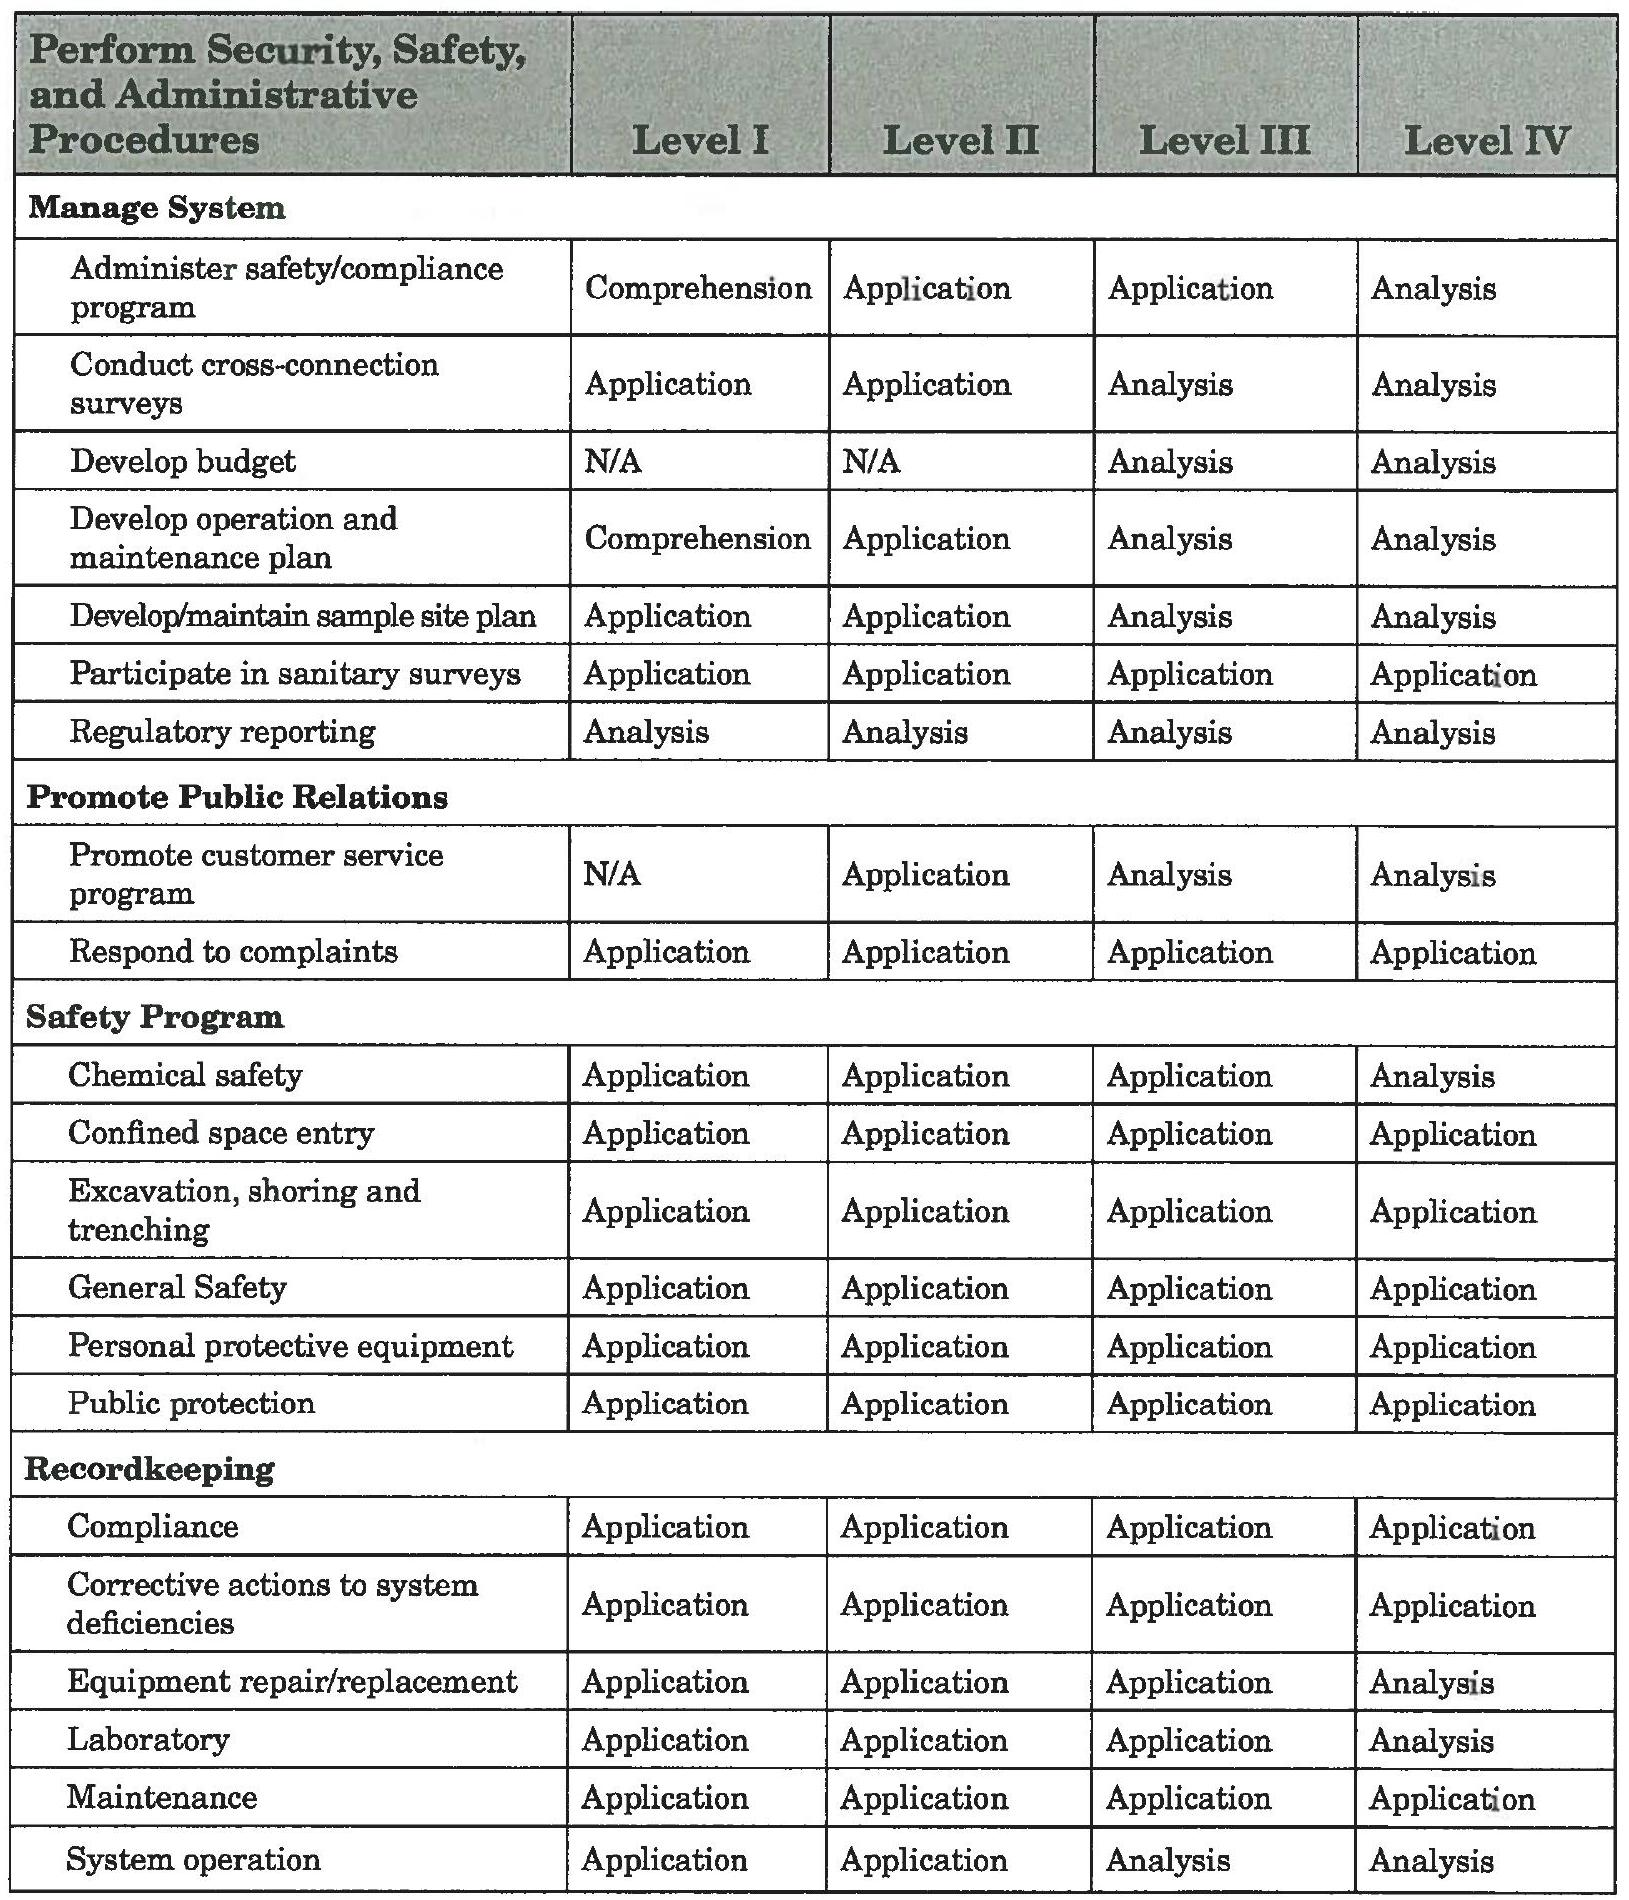
\includegraphics[max width=\textwidth]{2022_11_10_beeca89b60229885003dg-39}

\section{Required Capabillties}
\section{Knowledge of:}
\begin{itemize}
  \item Biological science

  \item Blueprint readings

  \item Building codes

  \item Data acquisition techniques

  \item Disciplinary procedures

  \item Emergency plans

  \item Employment laws

  \item Facility security

  \item Function of recordkeeping system

  \item General chemistry

  \item General electrical principles

  \item General hydraulic principles

  \item General mechanical principles

  \item Human resource practices

  \item Hydrology

  \item Local codes and ordinances

  \item Memorandums of understanding and agreements

  \item Monitoring requirements

  \item Potential causes of disasters in facility

  \item Potential impact of disasters in facility

  \item Principles of finance

  \item Principles of general communication

  \item Principles of management

  \item Principles of measurement

  \item Principles of public relations

\end{itemize}

\section{Abillty to:}
\begin{itemize}
  \item Assess likelihood of disaster occurring

  \item Assign work to proper trade

  \item Communicate in writing

  \item Communicate verbally

  \item Conduct meetings

  \item Conduct training programs

  \item Coordinate emergency response with other water organizations relative to the distribution system

  \item Determine what information needs to be recorded

  \item Develop a staffing plan

  \item Develop a work unit

  \item Evaluate facility performance

  \item Evaluate promotional materials

  \item Evaluate proposals

  \item Follow written procedures

  \item Generate a written safety program

  \item Generate capital plans - Principles of supervision

  \item Public notification requirements

  \item Public participation requirements

  \item Quality control/quality assurance practices

  \item Record keeping policies

  \item Regulations

  \item Reporting requirements

  \item Risk management

  \item Safe Drinking Water Act (SDWA)

  \item Sanitary spring design

  \item Sanitary survey processes

  \item Standards

  \item Water reuse

  \item Watershed management

  \item 40 CFR 141 Subpart A: General (definitions, coverage, variances and exemptions, siting requirements, and effective dates)

  \item 40 CFR 141 Subpart D: Reporting and Recordkeeping Requirements

  \item 40 CFR 141 Subpart O: Consumer Confidence Reports

  \item 40 CFR 141 Subpart Q: Public Notification of Drinking Water Violations

  \item Generate long- and short-term plans

  \item Identify potential safety hazards

  \item Interpret data

  \item Negotiate contracts

  \item Obtain unbiased data

  \item Organize information

  \item Perform distribution math

  \item Perform impact assessments

  \item Prepare proposals

  \item Recognize normal and abnormal analytical results

  \item Recognize unsafe work conditions

  \item Record information

  \item Review reports

  \item Select safety equipment

  \item Transcribe data

  \item Translate technical language into common terminology

  \item Write policies and procedures

\end{itemize}

\section{Perform Security, Safety, and Administrative Procedures}
\section{Sample Questions for Level I}
\section{Answers on page 351}
\begin{enumerate}
  \item Which agency sets legal limits on the concentration levels of harmful contaminants in potable water distributed to customers?\\
a. National Primary Drinking Water Regulations\\
b. United States Environmental Protection Agency\\
c. United States Public Health Service\\
d. Occupational Health and Safety Organization

  \item Which violations are the most serious?\\
a. Tier I\\
b. Tier II\\
c. Tier III\\
d. Tier IV

  \item A positive fecal coliform test must be reported to the primacy agency within\\
a. 8 hours.\\
b. 12 hours.\\
c. 24 hours.\\
d. 48 hours.

  \item The number of monthly distribution system bacteriological samples required is\\
a. based on water withdrawal permit limit.\\
b. based on system size.\\
c. based on population served.\\
d. different for each state.

  \item Which is the approximate angle of repose for average soils when using the sloping method for the prevention of cave-ins? (Note: horizontal to vertical distance, respectively)\\
a. $0.5: 1.0$\\
b. $1.0: 1.0$\\
c. $1.5: 1.0$\\
d. $2.0: 1.0$

\end{enumerate}

\section{Sample Questions for Level II}
\section{Answers on page 351}
\begin{enumerate}
  \item Which is the Maximum Contaminant Level for total trihalomethanes (TTHMs)?\\
a. $0.040 \mathrm{mg} / \mathrm{L}$\\
b. $\quad 0.060 \mathrm{mg} / \mathrm{L}$\\
c. $0.080 \mathrm{mg} / \mathrm{L}$\\
d. $0.100 \mathrm{mg} / \mathrm{L}$ 2. A system that fails to collect water samples in their distribution system would fall under which public notification requirement?\\
a. Tier I\\
b. Tier II\\
c. Tier III\\
d. Tier IV

  \item Under the Surface Water Treatment Rule, disinfection residuals must be collected at the same location in the distribution system as\\
a. coliform samples.\\
b. total trihalomethanes.\\
c. disinfection by-products.\\
d. alkalinity, conductivity, and $\mathrm{pH}$ for corrosion studies.

  \item Iron can cause "red water" and thus customer complaints when its concentration is above its secondary maximum contaminant level of\\
a. $0.01 \mathrm{mg} / \mathrm{L}$.\\
b. $\quad 0.05 \mathrm{mg} / \mathrm{L}$.\\
c. $0.10 \mathrm{mg} / \mathrm{L}$.\\
d. $0.30 \mathrm{mg} / \mathrm{L}$.

  \item Which chemical may encourage the growth of algae and microorganisms?\\
a. Lime\\
b. Sodium bicarbonate\\
c. Sodium hydroxide\\
d. Zinc orthophosphate

\end{enumerate}

\section{Sample Questlons for Level III}
\section{Answers on page 351}
\begin{enumerate}
  \item Water systems that collect samples for coliform testing must not find more than percentage of the samples they collect each month to be coliform positive.\\
a. $2 \%$\\
b. $4 \%$\\
c. $5 \%$\\
d. $10 \%$

  \item Which is the Maximum Contaminant Level for nitrate as measured as nitrogen?\\
a. $1.0 \mathrm{mg} / \mathrm{L}$\\
b. $2.0 \mathrm{mg} / \mathrm{L}$\\
c. $5.0 \mathrm{mg} / \mathrm{L}$\\
d. $10.0 \mathrm{mg} / \mathrm{L}$

  \item How much time does a community water system have for public notification if they have any Tier III violation?\\
a. 60 days\\
b. 3 months\\
c. 6 months\\
d. 12 months 4. Cohesive soil would contain a lot of\\
a. water.\\
b. clay.\\
c. clay and silt.\\
d. clay, silt, and sand.

  \item The lead and copper rule requires lead to be less than $0.015 \mathrm{mg} / \mathrm{L}$ in which percentage of the total samples collected?\\
a. $75 \%$\\
b. $90 \%$\\
c. $95 \%$\\
d. $99 \%$

\end{enumerate}

\section{Sample Questions for Level IV}
\section{Answers on page 352}
\begin{enumerate}
  \item Who should inspect the work of a water storage painting contractor?\\
a. The water utility supervisor\\
b. A water operator or operators responsible for the area the tank is located in\\
c. At least two competing painting contractors\\
d. A qualified third party

  \item Aviation warning lights on water storage tanks have an FAA regulation that requires the bulbs to be replaced before they reach what percentage of their normal life expectancy?\\
a. $50 \%$\\
b. $60 \%$\\
c. $75 \%$\\
d. $80 \%$

  \item The most expensive part of a pipe installation is/are the\\
a. pipe fittings.\\
b. valves.\\
c. excavation.\\
d. engineers' design.

  \item Which of the following is a potential biological biotoxin threat?\\
a. Sarin\\
b. Ricin\\
c. Taban\\
d. 3-quinucli dinyl benzilate

  \item The IDLH (Immediately Dangerous to Life and Health) value for chlorine, set by the National Institution of Occupational Safety and Health, is\\
a. $10 \mathrm{ppm}$.\\
b. $15 \mathrm{ppm}$.\\
c. $25 \mathrm{ppm}$.\\
d. $30 \mathrm{ppm}$.

\end{enumerate}

\section{Additional Distribution Operator Practice Questions}
\section{Answers on page 353}
\begin{enumerate}
  \item At which time of day is the age of the water stored in the distribution system the lowest?\\
a. Early morning\\
b. Late morning\\
c. Early afternoon\\
d. Late evening

  \item Which type of maps should not overlap each other?\\
a. Index maps\\
b. Comprehensive maps\\
c. Construction maps\\
d. Sectional maps

  \item Which one of the following is a type of joint for ductile iron piping?\\
a. Welded joint\\
b. Expansion joint\\
c. Flexible ball joint\\
d. Bell and spigot with rubber o-ring

  \item The amount of energy in feet required to overcome resistance to flow in a pipe is called\\
a. pump head.\\
b. cutoff head.\\
c. pressure head.\\
d. friction head.

  \item The fire insurance underwriters recommend that no main should have a diameter less than\\
a. 3 inches.\\
b. 4 inches.\\
c. 6 inches.\\
d. 8 inches.

  \item Water velocities through pipe should be limited to $5 \mathrm{ft} / \mathrm{sec}$ in order to\\
a. minimize friction loss.\\
b. reduce the number of pressure reducing stations.\\
c. minimize destruction of piping appurtenances.\\
d. reduce the amount of corrosion inhibitors applied to piping. 7. Which of the following is a type of joint for polyvinyl chloride piping?\\
a. Bell and spigot type\\
b. Thermal butt-fusion\\
c. Expansion joint\\
d. Restrained joint

  \item Which of the following is a type of joint for high-density polyethylene piping?\\
a. Bell and spigot type\\
b. Thermal butt-fusion\\
c. Push-on joint\\
d. Restrained joint

  \item Which of the following is a type of joint for ductile iron piping?\\
a. Welded joint\\
b. Restrained joint\\
c. Expansion joint\\
d. Rubber gasket joint

  \item Which of the following is a type of joint for ductile iron piping?\\
a. Welded joint\\
b. Bell and spigot joint\\
c. Expansion joint\\
d. Flanged joint

  \item The height of water in three differently shaped tanks is $22.4$ feet. Which tank will have the highest psi at the bottom?\\
a. The square tank\\
b. The rectangular tank\\
c. The cylindrical tank\\
d. It will be the same in all three tanks

  \item A water tank has a glass tube on its side showing the water level in the tank. What is this surface called?\\
a. Hydraulic grade line\\
b. Piezometric surface\\
c. Potentiometric surface\\
d. Potential surface

  \item Minor head losses are caused by\\
a. slime growths and corrosion or scaling.\\
b. corrosion and tuberculation.\\
c. type of pipe material and "C" factor.\\
d. sudden changes in direction or velocity of flow.

  \item Water mains should primarily be sized based on\\
a. earthquake size potential.\\
b. peak domestic and commercial demands.\\
c. peak commercial and industrial demands.\\
d. adequate fire flow at an appropriate pressure. 15. The most desirable residential pressure ranges from\\
a. 20 to 35 psi.\\
b. 35 to 50 psi.\\
c. 50 to 75 psi.\\
d. 75 to 90 psi.

  \item Which is pipe strength expressed in?\\
a. Hydrostatic potential\\
b. Psi and durability\\
c. Tensile and flexural strength\\
d. Baud units

  \item The resistance of a material to longitudinal pulling forces before it breaks is called\\
a. flexural strength.\\
b. shear strength.\\
c. ductile strength.\\
d. tensile strength.

  \item Most water systems use hydrants with two nozzles with diameters of and one nozzle with a diameter of\\
a. $2.0$ inches; $3.0$ inches\\
b. $2.0$ inches; $4.0$ inches\\
c. $2.5$ inches; $3.5$ inches\\
d. $2.5$ inches; $4.5$ inches

  \item Which type of pipe is durable and strong, has high flexural strength and good corrosion resistance, and is easily tapped?\\
a. High-density polyethylene\\
b. Steel\\
c. Ductile iron\\
d. Reinforced concrete

  \item Which of the following is a type of joint for concrete piping?\\
a. Expansion joint\\
b. Push-on joint\\
c. Bell and spigot type\\
d. Flanged joint

  \item Precipitative softening water treatment plants try to end up with distribution system water that is\\
a. slightly scale forming.\\
b. moderate scale forming.\\
c. neutral.\\
d. in equilibrium.

  \item Which is a closed fire line?\\
a. Broken fire hydrant or pipeline that feeds a fire hydrant\\
b. Unmetered connection for a fire protection system\\
c. Closed valve to a fire hydrant\\
d. Closed valve to a fire sprinkler system 23. Comprehensive maps of medium to large systems generally have scales ranging from\\
a. 250 to 500 feet to 1 inch.\\
b. 500 to 1,000 feet to 1 inch.\\
c. 1,000 to 1,500 feet to 1 inch.\\
d. 1,500 to 2,000 feet to 1 inch.

  \item Sectional maps generally have scales ranging from\\
a. 50 to 100 feet to 1 inch.\\
b. 100 to 200 feet to 1 inch.\\
c. 200 to 250 feet to 1 inch.\\
d. 250 to 400 feet to 1 inch.

  \item Which type of centrifugal pumps are the most common?\\
a. Axial flow impellers\\
b. Radial fow impellers\\
c. Mixed flow impellers\\
d. Vertical flow impellers

  \item Which of the following is a type of joint for steel piping?\\
a. Flexible ball joint\\
b. Restrained joint\\
c. Expansion joint\\
d. Push-on joint

  \item Which of the following is a type of joint for steel piping?\\
a. Flexible ball joint\\
b. Rubber gasket joint\\
c. Restrained joint\\
d. Galvanized steel ring

  \item The pressure during fire flow conditions should not drop below\\
a. 15 psi.\\
b. 20 psi.\\
c. 25 psi.\\
d. 30 psi.

  \item During a fire flow event, the residual pressure in a large main should be greater than\\
a. 15 psi.\\
b. 20 psi.\\
c. 25 psi.\\
d. 35 psi.

  \item Which type of distribution system configuration has smaller mains that generally terminate as dead-ends?\\
a. Grid system\\
b. Dendritic system\\
c. Arterial-loop system\\
d. Tree system 31. Which is applied to electrodes placed in the water of a water storage tank?\\
a. AC current\\
b. DC current\\
c. An electrolytic inhibitor around the seals where the wires enter the electrodes\\
d. Nothing

  \item The frequent starting of distribution system pumps probably indicates\\
a. pump is overheating.\\
b. inadequate supply to pump or check valve leaking back.\\
c. inadequate distribution storage.\\
d. pump is in need of maintenance.

  \item Which needs to be determined first when designing a pump station?\\
a. Discharge requirements\\
b. Head requirements\\
c. Power requirements\\
d. Capacity requirements

  \item Which is plotted on the horizontal scale (x-axis) of a pump curve?\\
a. Efficiency\\
b. Capacity (flow rate)\\
c. Total head\\
d. Power

  \item Hydraulics is the study of\\
a. fluid pressure in pipes or conduits.\\
b. the force of fluids in motion.\\
c. the pressure of fluids in motion.\\
d. fluids in motion and at rest.

  \item Which type of pipe joint consists of two machined surfaces?\\
a. Restrained joint\\
b. Push-on joint\\
c. Flanged joint\\
d. Mechanical joint

  \item Which type of pipe joint requires a movable follower ring?\\
a. Flanged joint\\
b. Grooved joint\\
c. Restrained joint\\
d. Mechanical joint

  \item What is the height limit to which siphoned water can be lifted at sea level?\\
a. $22.4$ feet\\
b. $32.0$ feet\\
c. $33.9$ feet\\
d. $34.0$ feet 39. How many feet of water will equal the atmospheric pressure at sea level?\\
a. 28\\
b. 30\\
c. 32\\
d. 34

  \item Which type of impeller is best to use for pumping water with low volumes of solids?\\
a. Closed\\
b. Open\\
c. Semi-open\\
d. Radial

  \item Which type of pump has the ability to rotate its discharge $360^{\circ}$ ?\\
a. End suction pump\\
b. Split case pump\\
c. Vertical pump\\
d. Jet pump

  \item How many times higher than the normal operating pressure should the pressure rating of distribution system piping be?\\
a. $1.0$ to $2.0$ times\\
b. $2.5$ to $4.0$ times\\
c. $4.0$ to $5.0$ times\\
d. $5.0$ to $7.0$ times

  \item Which type of pipe has been banned in the water industry?\\
a. Ductile iron\\
b. Steel\\
c. Asbestos cement\\
d. High-density polyethylene

  \item Which of the following types of pipe comes in diameters as large as 168 inches (14 feet)?\\
a. Cast-iron pipe\\
b. Reinforced concrete\\
c. Ductile iron\\
d. Prestressed concrete

  \item Which type of pipe has the highest normal maximum working pressure?\\
a. Reinforced concrete\\
b. Ductile iron\\
c. Polyvinyl chloride\\
d. High-density polyethylene

  \item Which type of pipe has the lowest normal maximum working pressure?\\
a. Reinforced concrete\\
b. Ductile iron\\
c. Polyvinyl chloride\\
d. High-density polyethylene 47. Ductile iron piping using flexible ball joints is most appropriate for\\
a. low-pressure applications.\\
b. high-pressure applications.\\
c. river crossings or rugged terrain.\\
d. all locations.

  \item Ductile iron piping using push-on or mechanical joints is most appropriate\\
a. for low-pressure applications.\\
b. for high-pressure applications.\\
c. for river crossings or rugged terrain.\\
d. where flexibility is required.

  \item Polyvinyl chloride piping using solvent weld joints is most appropriate\\
a. only for small lines.\\
b. for high pressure applications.\\
c. where flexibility is required.\\
d. where valves or fittings are to be attached.

  \item Concrete piping using bell and spigot type joints is appropriate\\
a. for all locations.\\
b. where expansion or contraction will occur.\\
c. under low-pressure applications.\\
d. under high-pressure applications.

  \item Which type of pipe joint is available in both bolted and boltless flexible pipe joint designs?\\
a. Ball and socket joint\\
b. Push-on joint\\
c. Grooved joint\\
d. Shouldered joint

  \item Which type of pipe joint permits flexible pipe alignment, is inexpensive to manufacture, and is easy to assemble?\\
a. Mechanical joint\\
b. Push-on joint\\
c. Grooved joint\\
d. Ball and socket joint

  \item Which type of pipe joint has machined ends?\\
a. Restrained joint\\
b. Flanged joint\\
c. Mechanical joint\\
d. Shouldered joint

  \item New polyvinyl chloride pipe has a C-value of about\\
a. 125 .\\
b. 125 to 128 .\\
c. 135 .\\
d. $150+$. 55. Which of the following water storage facilities is most likely to contain non-potable water?\\
a. Standpipe\\
b. Buried storage tanks\\
c. Emergency storage tanks\\
d. Elevated tanks using a riser; one way in and one way out

  \item Which type of valve is used on hydraulic lines connected to valve actuators?\\
a. Pinch valve\\
b. Needle valve\\
c. Pressure-relief valve\\
d. Vacuum-relief valve

  \item Which type of valve would be particularly useful for throttling the flow of corrosive liquids?\\
a. Diaphragm valve\\
b. Butterfly valve\\
c. Gate valve\\
d. Pinch valve

  \item Water meter pits are usually used in\\
a. areas where flooding will most likely occur.\\
b. areas where flooding is very rare.\\
c. cold climates.\\
d. hot climates.

  \item A horizontal load, parallel to a pump shaft is called a\\
a. shear load.\\
b. thrustload.\\
c. radial load.\\
d. stress load.

  \item Manufacturers typically design pumps such that the first critical speed is at least higher or lower than rated speed.\\
a. $10 \%$\\
b. $20 \%$\\
c. $25 \%$\\
d. $30 \%$

  \item Regarding fire flow, mains smaller than 6 inches should only be used\\
a. in residential areas.\\
b. in low-value districts.\\
c. in rural areas.\\
d. to complete a grid.

  \item Which type of pipe requires special external protection in high-chloride soils?\\
a. Reinforced concrete\\
b. Ductile iron\\
c. Steel\\
d. High-density polyethylene 63. Which type of pipe would most likely collapse or become distorted under a partial vacuum?\\
a. Asbestos-cement\\
b. Steel\\
c. Cast iron\\
d. Plastic

  \item Casing pipe used to house a large water main under a railroad crossing should have a diameter that is larger than the outside diameter of the water main bells.\\
a. less than 2 inches\\
b. 2 to 8 inches\\
c. 8 to 6 inches\\
d. 6 to 8 inches

  \item Data manipulations using the basic elements of an automatic mapping (MS)/Facility mapping (FM)/Geographic Information Systems (GIS) would include\\
a. collection and storage.\\
b. collection and management.\\
c. modeling and analysis.\\
d. retrieval, display, and storage.

  \item Which data category for water utility data sets includes the following map layers: Control information, planimetric features, and hydrology features?\\
a. Land records data\\
b. Natural resources data\\
c. Watershed resources data\\
d. Base data

  \item Which of the following chlorine species is called $\mathrm{HTH}$ ?\\
a. Hypochlorous acid\\
b. Sodium hypochlorite\\
c. Calcium hypochlorite\\
d. Hypotrichloro-hydrocarbon

  \item Which is the proper detention time for disinfecting a water storage tank that is filled with already chlorinated water such that the free chlorine residual is $10 \mathrm{mg} / \mathrm{L}$ after the proper detention time is completed?\\
a. 4 hours\\
b. 6 hours\\
c. 8 hours\\
d. 24 hours

  \item Which is the proper detention time for disinfecting a water storage tank with water that is mixed with hypochlorite already in the tank such that the free chlorine is $10 \mathrm{mg} / \mathrm{L}$ after proper detention time is complete?\\
a. 6 hours\\
b. 8 hours\\
c. 12 hours\\
d. 24 hours 70. The disinfectant residual in treated water entering the distribution system must not be less than\\
a. $\quad 0.2 \mathrm{mg} / \mathrm{L}$ at anytime.\\
b. $\quad 0.2 \mathrm{mg} / \mathrm{L}$ for more than 4 hours during periods when the system is serving water to the public.\\
c. $\quad 0.4 \mathrm{mg} / \mathrm{L}$ at anytime.\\
d. $0.4 \mathrm{mg} / \mathrm{L}$ for more than $5 \%$ of the time that the system is serving water to the public.

  \item The chemical formula for Hypochlorous acid is\\
a. $\mathrm{OCl}^{-}$.\\
b. $\mathrm{NaOCl}$.\\
c. $\mathrm{HOCl}$.\\
d. $\mathrm{Ca}(\mathrm{OCl})_{2}$.

  \item Usually the best disinfectant to use in large-diameter pipes or very long pipelines is\\
a. calcium hypochlorite.\\
b. sodium hypochlorite.\\
c. chlorine gas.\\
d. chloramines.

  \item Which method for controlling nitrification problems in a distribution system would result in a temporary increase in trihalomethanes?\\
a. Increasing the chlorine to nitrogen weight ratio\\
b. Superchlorinating reservoirs and storage tanks\\
c. Decreasing chlorine detention time in reservoirs and distribution pipelines\\
d. Flushing the distribution pipelines

  \item Which is the available chlorine concentration used for disinfecting a water storage tank using a method that involves spraying or painting of all the interior tank surfaces?\\
a. $50 \mathrm{mg} / \mathrm{L}$\\
b. $100 \mathrm{mg} / \mathrm{L}$\\
c. $200 \mathrm{mg} / \mathrm{L}$\\
d. $250 \mathrm{mg} / \mathrm{L}$

  \item When following a two-step process for disinfecting a water storage tank, the initial dosage of $50 \mathrm{mg} / \mathrm{L}$ available chlorine should be held in the partially filled tank for\\
a. at least 6 hours.\\
b. at least 10 hours.\\
c. at least 24 hours.\\
d. at least 3 days.

  \item Why are altitude valves used on water storage tanks?\\
a. To allow water to pass in and out of the tank as pressure fluctuates\\
b. To stop the flow of water into the tank when it is full\\
c. To allow overflow water to flow out of the tank\\
d. To shut the flow of water to the tank off for maintenance and inspection 77. If iron bacteria are causing corrosion problems in the distribution system, which is the most probable solution?\\
a. Flushing\\
b. Use a corrosion chemical as treatment\\
c. Use a surfactant dispersion chemical\\
d. Acidify the system, then flush

  \item Which type of chlorine gas feeder is most commonly used?\\
a. Pressure\\
b. Combination water and pressure\\
c. Vacuum\\
d. Combination pressure and vacuum

  \item When concentration cell corrosion occurs in iron pipes the electrons will move through the\\
a. water from the anode to the cathode.\\
b. water from the cathode to the anode.\\
c. iron pipe from the anode to the cathode.\\
d. iron pipe from the cathode to the anode.

  \item Which type of corrosion occurs when two dissimilar metals are electrically connected and immersed in a common flow of water, where one metal becomes the anode and the other the cathode?\\
a. Concentration cell corrosion\\
b. Localized corrosion\\
c. Uniform corrosion\\
d. Galvanic corrosion

  \item Which is the main purpose(s) of the meter yoke?\\
a. Cushion against stress\\
b. Cushion against stress and strain\\
c. Provide electrical conductivity\\
d. Proper alignment and support for meter

  \item The minimum cover over a water main below a road in a warm climate with no possibility of frost is\\
a. $2.0$ feet.\\
b. $2.5$ feet.\\
c. $3.0$ feet.\\
d. $3.5$ feet.

  \item The minimum cover over a water service below a road in a warm climate with no possibility of frost is\\
a. 12 inches.\\
b. 18 inches.\\
c. 24 inches.\\
d. 30 inches. 99. What is the maximum joint deflection for full lengths of standard 48-inch ductileiron push-joint pipe?\\
a. 3 degrees\\
b. 6 degrees\\
c. 8 degrees\\
d. 10 degrees

  \item Large meters are usually tested at which percentage of their operating range?\\
a. 5 to $10 \%$\\
b. 10 to $20 \%$\\
c. 20 to $25 \%$\\
d. 25 to $33 \%$

  \item Which one of the following types of pipe is most prone to sliding out of a push-on joint if not firmly restrained?\\
a. Asbestos-cement pipe\\
b. Plastic pipe\\
c. Ductile-iron pipe\\
d. Cast-iron pipe

  \item Which is the best mechanical compacting equipment for deep narrow trenches?\\
a. Hand-controlled plate tampers\\
b. Vibratory compactors\\
c. Irregular drum tampers\\
d. Boom-mounted plate tampers

  \item The lantern ring is also known as the\\
a. packing ring.\\
b. seal cage.\\
c. packing seal.\\
d. mechanical seal.

  \item How is the capacity of a centrifugal pump related to total head?\\
a. Directly\\
b. Indirectly\\
c. Linear\\
d. Disproportionately

  \item The bearings that maintain the radial positioning of a shaft are called\\
a. radial bearings.\\
b. rolling bearings.\\
c. sleeve bearings.\\
d. thrust bearings.

  \item When the discharge of a velocity pump is blocked, head builds up, typically greater than the pressure generated during pumping. When this occurs, water recirculates within the pump impeller and casing. This flow condition is called\\
a. run-around.\\
b. skirting.\\
c. slip.\\
d. bypass. 107. Which valves can be used to throttle flow for only a short period of time?\\
a. Butterfly valves\\
b. Altitude valves\\
c. Self-actuating valves\\
d. Plug valves

  \item Which type of valve operates similar to a diaphragm valve?\\
a. Vacuum relief valve\\
b. Globe valve\\
c. Pressure relief valve\\
d. Butterfly valve

  \item Which valve can go from fully open to fully closed with $1 / 4$ turn?\\
a. Plug valve\\
b. Needle valve\\
c. Globe valve\\
d. Pinch valve

  \item Foot valves are a special type of\\
a. relief valve.\\
b. control valve.\\
c. check valve.\\
d. plug valve.

  \item Usually, which type of hydrant is a flush hydrant?\\
a. Warm-climate hydrant\\
b. Wet-barrel hydrant\\
c. Dry-barrel hydrant\\
d. Standpipe-barrel hydrant

  \item Which type of temperature sensor uses two wires of different materials?\\
a. Thermistors\\
b. Thermo-resistors\\
c. Thermocouples\\
d. Thermo-conductors

  \item Which type of temperature sensor uses a semi-conductive material?\\
a. Thermistors\\
b. Thermo-resistors\\
c. Thermocouples\\
d. Thermo-conductors

  \item The amount of energy in feet that a pump supplies to a fluid is called\\
a. velocity head.\\
b. pump head.\\
c. total head.\\
d. pressure head. 115. Which is the most frequent cause of hydraulic transients in water distribution systems?\\
a. Controlled pump shutdown\\
b. Flow demand changes\\
c. Pump startup\\
d. Valve opening and closing

  \item Which type of valve should be used for filling an elevated tank if full system pressure would overflow the tank?\\
a. Pressure-relief valve\\
b. Altitude valve\\
c. Pressure-reducing valve\\
d. Globe valve

  \item One form of a differential-pressure flow meter is $a(n)$\\
a. propeller.\\
b. proportional.\\
c. velocity-type.\\
d. orifice plate.

  \item If a centrifugal pump with a single volute is operated at more than of its design capacity, an excess radial load will result, causing premature bearing failure.\\
a. $110 \%$\\
b. $120 \%$\\
c. $125 \%$\\
d. $135 \%$

  \item How many inches of mercury is a total vacuum at sea level?\\
a. $14.7$ inches\\
b. $30.0$ inches\\
c. $34.0$ inches\\
d. $39.6$ inches

  \item How many feet of water will equal the atmospheric pressure at sea level?\\
a. 28 feet\\
b. 30 feet\\
c. 32 feet\\
d. 34 feet

  \item Pressure gauges connected to both suction and discharge sides of a pump should be connected\\
a. 2 to 3 feet on either side of a pump, unless there is a change in direction it can go closer.\\
b. 1 foot and 2 feet from the pump on the suction side and discharge side, respectively.\\
c. next to the pump on the suction side and just before the check valve on the discharge valve.\\
d. to the pressure taps supplied on the pump. 122. Which are the two principal types of throttling valves?\\
a. Throttling and pressure-reducing valves\\
b. Butterfly and relief valves\\
c. Butterfly and altitude valves\\
d. Pressure-reducing and altitude valves

  \item Which valve would be best to use to precisely throttle flow?\\
a. Globe valve\\
b. Butterfly valve\\
c. Rotary valve\\
d. Needle valve

  \item SCADA systems consist of the following distinct components:\\
a. Remote terminal units (RTUs), communications, and human machine interface (HMI)\\
b. Sensing instrument, RTUs, communications, and HMI\\
c. Sensing instrument, RTUs, communications, master station, and HMI\\
d. RTUs, communications, master station, and HMI

  \item Stray-current corrosion is caused by\\
a. corrosive soils.\\
b. acidic soils.\\
c. AC currents.\\
d. DC currents.

  \item When a metal is galvanized, it is coated with\\
a. zinc.\\
b. aluminum.\\
c. aluminum oxide.\\
d. aluminum hydroxide.

  \item Which system would provide for a "soft start" to a motor?\\
a. Wound-rotor induction motor and a controller\\
b. Synchronous motor and a variable frequency controller\\
c. A variable frequency drive and a squirrel-cage induction motor\\
d. Squirrel-cage induction drive and a variable frequency drive

  \item Which type of relay is frequently used to detect power loss and initiate a switchover to another power source?\\
a. Loss-of-phase relays\\
b. Voltage relays\\
c. Frequency relays\\
d. Circuit breaker relays

  \item Which type of relays are placed on each phase of a power supply to open up a control circuit and stop a motor, if the current becomes excessive?\\
a. Thermal-overload relays\\
b. Frequency relays\\
c. Voltage relays\\
d. Differential relays 130. Which type of relay is often used where local power generation is involved and on synchronous motor starters to sense when the motor has reached synchronizing speed?\\
a. Speed sensor relay\\
b. Differential relay\\
c. Frequency relay\\
d. Voltage relay

  \item Which type of relay is frequently used on large equipment to check whether all the current entering a system comes back out of the system?\\
a. Voltage relay\\
b. Over-current relay\\
c. Reverse-current relay\\
d. Differential relay

  \item Which is the correct sequence of a telemetry signal?\\
a. Indicator, sensor, transmission channel, receiver, transmitter, and signal\\
b. Sensor, transmitter, transmission channel, receiver, and indicator\\
c. Signal, indicator, transmitter, transmission channel, receiver, and sensor\\
d. Signal, sensor, transmission channel, transmitter, receiver, and indicator

  \item Which type of instrument is used to measure the average power of a load over a specific time interval?\\
a. Demand meter\\
b. Voltmeter\\
c. Ammeter\\
d. Wattmeter

  \item Sacrificial anodes are also called\\
a. corrosion anodes.\\
b. corrosion cells.\\
c. galvanic anodes.\\
d. decaying anodes.

  \item Which is becoming the most common, and is one of the least dangerous, methods of thawing a water service line?\\
a. Hot water\\
b. Electrical\\
c. Small torch\\
d. Steam vibration

  \item When a control switch operated by pressure changes is located too close to a pump station, erratic operation can occur. This problem is known as\\
a. pulsing.\\
b. seesaw arching.\\
c. racking.\\
d. roaming. 137. Which is the electronic standard range?\\
a. 4 to $20 \mathrm{~mA} \mathrm{DC}$\\
b. 4 to $20 \mathrm{~mA} \mathrm{AC}$\\
c. 0 to $100 \%$\\
d. 0 to 1 binary

  \item Which is the chemical makeup of a tubercle?\\
a. $\mathrm{Mn}(\mathrm{OH})_{2}$ on the inside and $\mathrm{Ca}\left(\mathrm{HCO}_{3}\right)_{2}$ on the outside\\
b. $\mathrm{Mn}(\mathrm{OH})_{2}$ on the outside and $\mathrm{Ca}\left(\mathrm{HCO}_{3}\right)_{2}$ on the inside\\
c. $\mathrm{Fe}(\mathrm{OH})_{2}$ on the inside and $\mathrm{Fe}\left(\mathrm{OH}_{3}\right)$ on the outside\\
d. $\mathrm{Fe}(\mathrm{OH})_{2}$ on the outside and $\mathrm{Fe}\left(\mathrm{OH}_{3}\right)$ on the inside

  \item Which device consists of a pair of metallic plates that are separated by an insulating material called a dielectric?\\
a. Storage battery\\
b. Voltage regulator\\
c. Rectifier\\
d. Capacitor

  \item The current rating of a fuse should be the current rating of the circuit or device that it protects.\\
a. slightly lower than\\
b. $15 \%$ greater than\\
c. equal to\\
d. equal to or slightly larger than

  \item Conductors usually fail because of\\
a. excessive heat.\\
b. mechanical failure.\\
c. lightening.\\
d. simple aging.

  \item Inspection of the shaft and coupling alignment should be performed every or immediately, if problem signs develop.\\
a. month\\
b. quarter\\
c. 6 months\\
d. year

  \item Bearings should not be lubricated with this type of oil because this oil forms acids as it begins to break down.\\
a. Non-detergent mineral oil\\
b. Animal oil\\
c. SAE 10\\
d. SAE 20

  \item How much resistance should motor-winding insulation exhibit?\\
a. At least $0.5$ megohm of resistance\\
b. At least $1.0$ megohm of resistance\\
c. At least $2.0$ megohm of resistance\\
d. At least $5.0$ megohm of resistance 145. Which is the pneumatic standard range?\\
a. 0 to 10 psig\\
b. 3 to 15 psig\\
c. 4 to 20 psig\\
d. 0 to $100 \%$

  \item Which of the following methods for preventing external corrosion is only a shortterm remedy?\\
a. Extra thickness for pipe walls\\
b. Wrapping pipe in polyethylene plastic sleeves\\
c. Applying a coating of bitumastic or coal tar\\
d. Installing cathodic protection on the pipe

  \item The D'Arsonval meter is\\
a. an amperometric meter.\\
b. a type of $\mathrm{pH}$ meter.\\
c. an analog (uses a needle) meter.\\
d. a digital (number displays on unit) meter.

  \item How does $\mathrm{H}_{2} \mathrm{~S}$ gas kill a person?\\
a. Asphyxiation\\
b. Paralyzes the respiratory system\\
c. Paralyzes the nervous system\\
d. Stops the heart

  \item If sodium hypochlorite comes into contact with the skin, it should be immediately flushed with water for at least\\
a. 10 minutes\\
b. 15 minutes\\
c. 20 minutes\\
d. 30 minutes

  \item Which is the Secondary Maximum Contaminant Level for $\mathrm{pH}$ ?\\
a. $7.0 \mathrm{pH}$ units\\
b. $\quad 6.5$ to $7.5 \mathrm{pH}$ units\\
c. $6.5$ to $8.5 \mathrm{pH}$ units\\
d. $6.0$ to $8.5 \mathrm{pH}$ units

  \item If an excavation on a road requires that one of the lanes be closed and the speed limit is $25 \mathrm{mph}$, how many cones are required to divert the traffic?\\
a. 6\\
b. 9\\
c. 13\\
d. 15

  \item If an excavation on a road requires that one of the lanes be closed and the speed limit is $45 \mathrm{mph}$, how many cones are required to divert the traffic?\\
a. 9\\
b. 13\\
c. 15\\
d. 18 137. Which is the electronic standard range?\\
a. 4 to $20 \mathrm{~mA} \mathrm{DC}$\\
b. 4 to $20 \mathrm{~mA} A C$\\
c. 0 to $100 \%$\\
d. 0 to 1 binary

  \item Which is the chemical makeup of a tubercle?\\
a. $\mathrm{Mn}(\mathrm{OH})_{2}$ on the inside and $\mathrm{Ca}\left(\mathrm{HCO}_{3}\right)_{2}$ on the outside\\
b. $\mathrm{Mn}(\mathrm{OH})_{2}$ on the outside and $\mathrm{Ca}\left(\mathrm{HCO}_{3}\right)_{2}$ on the inside\\
c. $\mathrm{Fe}(\mathrm{OH})_{2}$ on the inside and $\mathrm{Fe}\left(\mathrm{OH}_{3}\right)$ on the outside\\
d. $\mathrm{Fe}(\mathrm{OH})_{2}$ on the outside and $\mathrm{Fe}\left(\mathrm{OH}_{3}\right)$ on the inside

  \item Which device consists of a pair of metallic plates that are separated by an insulating material called a dielectric?\\
a. Storage battery\\
b. Voltage regulator\\
c. Rectifier\\
d. Capacitor

  \item The current rating of a fuse should be the current rating of the circuit or device that it protects.\\
a. slightly lower than\\
b. $15 \%$ greater than\\
c. equal to\\
d. equal to or slightly larger than

  \item Conductors usually fail because of\\
a. excessive heat.\\
b. mechanical failure.\\
c. lightening.\\
d. simple aging.

  \item Inspection of the shaft and coupling alignment should be performed every or immediately, if problem signs develop.\\
a. month\\
b. quarter\\
c. 6 months\\
d. year

  \item Bearings should not be lubricated with this type of oil because this oil forms acids as it begins to break down.\\
a. Non-detergent mineral oil\\
b. Animal oil\\
c. SAE 10\\
d. SAE 20

  \item How much resistance should motor-winding insulation exhibit?\\
a. At least $0.5$ megohm of resistance\\
b. At least $1.0$ megohm of resistance\\
c. At least $2.0$ megohm of resistance\\
d. At least $5.0$ megohm of resistance 145. Which is the pneumatic standard range?\\
a. 0 to 10 psig\\
b. 3 to 15 psig\\
c. 4 to 20 psig\\
d. 0 to $100 \%$

  \item Which of the following methods for preventing external corrosion is only a shortterm remedy?\\
a. Extra thickness for pipe walls\\
b. Wrapping pipe in polyethylene plastic sleeves\\
c. Applying a coating of bitumastic or coal tar\\
d. Installing cathodic protection on the pipe

  \item The D'Arsonval meter is\\
a. an amperometric meter.\\
b. a type of $\mathrm{pH}$ meter.\\
c. an analog (uses a needle) meter.\\
d. a digital (number displays on unit) meter.

  \item How does $\mathrm{H}_{2} \mathrm{~S}$ gas kill a person?\\
a. Asphyxiation\\
b. Paralyzes the respiratory system\\
c. Paralyzes the nervous system\\
d. Stops the heart

  \item If sodium hypochlorite comes into contact with the skin, it should be immediately flushed with water for at least\\
a. 10 minutes\\
b. 15 minutes\\
c. 20 minutes\\
d. 30 minutes

  \item Which is the Secondary Maximum Contaminant Level for $\mathrm{pH}$ ?\\
a. $7.0 \mathrm{pH}$ units\\
b. $\quad 6.5$ to $7.5 \mathrm{pH}$ units\\
c. $6.5$ to $8.5 \mathrm{pH}$ units\\
d. $6.0$ to $8.5 \mathrm{pH}$ units

  \item If an excavation on a road requires that one of the lanes be closed and the speed limit is $25 \mathrm{mph}$, how many cones are required to divert the traffic?\\
a. 6\\
b. 9\\
c. 13\\
d. 15

  \item If an excavation on a road requires that one of the lanes be closed and the speed limit is $45 \mathrm{mph}$, how many cones are required to divert the traffic?\\
a. 9\\
b. 13\\
c. 15\\
d. 18 153. Which chemical may cause leaching of lead in stagnant waters?\\
a. Sodium zinc phosphate\\
b. Lime\\
c. Sodium carbonate\\
d. Sodium hydroxide

  \item During simulated distribution testing, a borate buffer solution maintains a constant $\mathrm{pH}$ of\\
a. 10.\\
b. 8 .\\
c. 7 .\\
d. 5.

  \item In permit-entry confined space, who is responsible for terminating entries?\\
a. Authorized entrant\\
b. Standby attendant\\
c. Entry supervisor\\
d. Entry supervisor and the standby attendant

  \item In permit-entry confined space, who is responsible for summoning rescuers?\\
a. Standby attendant and authorized attendant\\
b. Entry supervisor and authorized attendant\\
c. Authorized attendant\\
d. Authorized entrant

  \item Extremely small chlorine leaks that go for weeks will most likely be found\\
a. by using a very strong ammonia solution.\\
b. by using soap and looking for bubbles.\\
c. by using your nose.\\
d. by seeing the discoloration and moisture at the leak point.

  \item Which is the Action Level for lead?\\
a. $0.015 \mathrm{mg} / \mathrm{L}$\\
b. $0.020 \mathrm{mg} / \mathrm{L}$\\
c. $0.025 \mathrm{mg} / \mathrm{L}$\\
d. $\quad 0.040 \mathrm{mg} / \mathrm{L}$

  \item Most regulated contaminants\\
a. are thought to cause liver or kidney damage.\\
b. can cause heart or cardiovascular diseases.\\
c. cause health effects only after long exposure.\\
d. cause acute effects.

  \item High levels of cadmium at the customer's tap would most likely be due to\\
a. copper pipe.\\
b. galvanized pipe.\\
c. iron pipe.\\
d. household fixtures. 161. Which is the Secondary Maximum Contaminant Level for zinc?\\
a. $1 \mathrm{mg} / \mathrm{L}$\\
b. $\quad 2 \mathrm{mg} / \mathrm{L}$\\
c. $5 \mathrm{mg} / \mathrm{L}$\\
d. $10 \mathrm{mg} / \mathrm{L}$

  \item The prevention of trench cave-ins using the sloping method requires which slope ratio? (Note: horizontal to vertical distance, respectively)\\
a. $1.0: 1.0$\\
b. $1.5: 1.0$\\
c. $2.0: 1.0$\\
d. The angle will vary with type of soil, moisture content, and surrounding conditions

  \item What is the Maximum Contaminant Level for asbestos fibers greater than 10 micrometers?\\
a. 1 million fibers per liter (MFL)\\
b. $2.5 \mathrm{MFL}$\\
c. $5.0 \mathrm{MFL}$\\
d. $7.0 \mathrm{MFL}$

  \item Which is the Locational Running Annual Average (LRAA) for trihalomethanes (THM) and haloacetic acid 5 (HAA5) under the Stage 2 Disinfectants/Disinfection By-Products Rule?\\
a. $80 / 60 \mu \mathrm{g} / \mathrm{L}$\\
b. $100 / 75 \mathrm{\mu g} / \mathrm{L}$\\
c. $100 / 80 \mu \mathrm{g} / \mathrm{L}$\\
d. $120 / 100 \mu \mathrm{g} / \mathrm{L}$

  \item Under the Surface Water Treatment Rule, undetected disinfection residuals must not exceed what percentage of samples each month for any two consecutive months that water is served to the public?\\
a. Zero tolerance\\
b. $1 \%$\\
c. $2 \%$\\
d. $5 \%$

  \item Which would be the most probable solution if Actinomycetes were causing taste and odor problems in the distribution system?\\
a. Use copper sulfate and flush the system\\
b. Start using chloramines as a disinfectant since it has a longer lasting residual compared to chlorine\\
c. Use activated carbon and flush the system\\
d. Control nutrients

  \item Where is scale most likely to form in a hypochlorinator?\\
a. Push rod\\
b. Plunger\\
c. Pump head\\
d. Spring 168. Which type of chlorine gas feeding equipment would be most appropriate for distribution systems where rechlorination is required?\\
a. Compound-loop control gas feeder\\
b. Automatic proportioning control gas feeder\\
c. Automatic residual control gas feeder\\
d. Semiautomatic control gas feeder

  \item When a sample is collected, its quality begins to change because of\\
a. dissolved gases.\\
b. chemical activity.\\
c. $\mathrm{pH}$.\\
d. alkalinity.

  \item Chemolithotrophic nitrifying bacteria are\\
a. gram-negative and anaerobic.\\
b. gram-positive and strictly aerobic.\\
c. gram-negative and facultative or aerobic.\\
d. gram-negative and strictly aerobic.

  \item Which index will indicate scale-forming water with values less than 6 and corrosive water with values greater than 7 ?\\
a. Baylis curve\\
b. Langelier saturation index\\
c. Marble test\\
d. Ryzner index

  \item The radiation term corresponding to an energy absorption of 100 ergs per gram of any medium is called a(n)\\
a. rad.\\
b. rem.\\
c. curie.\\
d. erg.

  \item Community and nontransient community water systems must test for if they use ozone for disinfection or oxidation.\\
a. chlorate\\
b. bromate\\
c. haloacetic acids (five)\\
d. total trihalomethanes

  \item According to AWWA Standard C652 Method 3, disinfection of water tanks requires exposure to free chlorine at a concentration of chlorine residual ending at a concentration of at least for 24-hours with the free\\
a. $10 \mathrm{mg} / \mathrm{L} ; 2 \mathrm{mg} / \mathrm{L}$\\
b. $25 \mathrm{mg} / \mathrm{L} ; 10 \mathrm{mg} / \mathrm{L}$\\
c. $50 \mathrm{mg} / \mathrm{L} ; 10 \mathrm{mg} / \mathrm{L}$\\
d. $100 \mathrm{mg} / \mathrm{L} ; 25 \mathrm{mg} / \mathrm{L}$ 175. If a main cannot be installed at an adequate depth in a cold weather climate, Styrofoam insulation board can be used to protect the water in the pipe from freezing. How far above the pipe should this insulation be installed?\\
a. 2 to 4 inches\\
b. 5 to 7 inches\\
c. 8 to 10 inches\\
d. 1 foot

  \item How much deeper below the grade line of a pipe bottom should a trench be excavated if it is being dug in a rock formation?\\
a. 3 to 6 inches\\
b. 6 to 9 inches\\
c. 9 to 12 inches\\
d. 12 to 18 inches

  \item Pressure-relief valves are most similar to\\
a. globe valves.\\
b. vacuum relief valves.\\
c. needle valves.\\
d. check valves.

  \item Current meters are primarily used for measuring flow in lines that are\\
a. $5 / 8$ to 1 inch.\\
b. 1 to 3 inches.\\
c. 3 inches or greater.\\
d. 12 inches or greater.

  \item Which does beam breakage resemble?\\
a. Shear breakage\\
b. Stress breakage\\
c. Flexural breakage\\
d. Tensile breakage

  \item Which type of valve should be installed for pressure control and flow control in large pipes?\\
a. Butterfly valve\\
b. Globe valve\\
c. Gate valve\\
d. Ball valve

  \item Which can be developed by measuring the pressure along a pipeline?\\
a. The C factor\\
b. The total dynamic head\\
c. The pipeline's grade\\
d. The hydraulic grade

  \item A thrust block would not be required on pipes that are\\
a. made of steel.\\
b. made of reinforced concrete.\\
c. welded at the joints.\\
d. of the bell and socket type. 183. Which is the recommended water pressure in commercial districts?\\
a. 50 to less than 65 psi\\
b. 55 to less than 75 psi\\
c. 75 to less than 100 psi\\
d. 90 to less than 120 psi

  \item Which can be used to avoid excessively high water pressures in distribution mains?\\
a. Pressure-reducing valves\\
b. Plug valves\\
c. Installation of a pneumatic tank\\
d. Blowoff valves

  \item Which is the commonly accepted water velocity in water mains at maximum flows?\\
a. 1 to $3 \mathrm{ft} / \mathrm{sec}$\\
b. 2 to $4 \mathrm{ft} / \mathrm{sec}$\\
c. 4 to $5 \mathrm{ft} / \mathrm{sec}$\\
d. 5 to $6 \mathrm{ft} / \mathrm{sec}$

  \item It is recommended that dead-end water mains more than 1,000 feet in length should be constructed of pipe that is at least in diameter.\\
a. 6 inches\\
b. 8 inches\\
c. 10 inches\\
d. 12 inches

  \item Water mains that are 12 inches or less in diameter should have isolation valves that are located not more than between each other.\\
a. 500 feet\\
b. 750 feet\\
c. 1,000 feet\\
d. 1,200 feet

  \item The size and capacity of a water distribution system is based largely on\\
a. peak hour customer demands.\\
b. fire demand.\\
c. agricultural demand.\\
d. industrial demand.

  \item A water storage tank located far from the source of demand would most likely have which type of problem during peak demand, if the area between storage and use is relatively flat?\\
a. Low flow due to friction losses\\
b. Poor water quality due to transmission pipe being too long\\
c. High pumping costs during peak hourly flow\\
d. Low pressure

  \item Which type of pipe material is prestressed?\\
a. Steel cylinder\\
b. Ductile iron\\
c. Asbestos-cement\\
d. C-900 PVC 191. Which type of service pipe material is no longer acceptable for drinking water?\\
a. Brass\\
b. Lead\\
c. Galvanized wrought iron\\
d. Copper

  \item Which type of joint for connecting water pipes has the advantage of moderate deflection and the gaskets used absorb vibration and pipe movement?\\
a. Flanged joint\\
b. Victaulic joint\\
c. Dressler coupling\\
d. Restrained joint

  \item Which type of joint for connecting water pipes has the disadvantage of having a grove that weakens the pipe wall?\\
a. Flanged joint\\
b. Victaulic joint\\
c. Dressler coupling\\
d. Restrained joint

  \item Which type of joint for connecting water pipes is used where the available space to lock a joint in place is lacking and where the soil behind the fitting may be disturbed?\\
a. Flanged joint\\
b. Victaulic joint\\
c. Dressler coupling\\
d. Restrained joint

  \item Which is normally used on the outside joint space of steel cylinder concrete in order to protect the joint rings from external corrosion?\\
a. Bituminous material\\
b. Epoxy material\\
c. Mastic coating\\
d. Cement mortar

  \item How much deflection is allowed for asbestos-cement couplings that are 3 to 12 inches in diameter?\\
a. 5 degrees\\
b. 7 degrees\\
c. 10 degrees\\
d. 12 degrees

  \item Which is the best or first choice corrosion control method(s) to protect pipe?\\
a. Use of noncorrosive metals and/or mechanical coatings\\
b. Chemical protective coatings\\
c. Electrical control by using cathodic protection\\
d. Use of metallic coatings such as zinc or aluminum 198. What is an effective way for a distribution system agency to measure financial stability?\\
a. Measuring the debt\\
b. Calculating the operating and coverage ratios\\
c. By dividing the paying customers by the total customers, then multiplying by $100 \%$; anything over $95 \%$ is excellent\\
d. Simply by how much money in the black that they have each fiscal year

  \item Where do good public relations start for a water utility?\\
a. With well-maintained fire hydrants\\
b. With meaningful advertising\\
c. Via public relations campaigns\\
d. Through dedicated service-oriented employees

  \item One of the most important functions and the major part of the work day for a manager of a water utility or distribution system is involved in\\
a. organizing.\\
b. planning.\\
c. directing.\\
d. controlling.

  \item Which term defines lead free, when used with respect to solders and flux?\\
a. Containing not more than $0.01 \%$ lead\\
b. Containing not more than $0.02 \%$ lead\\
c. Containing not more than $0.04 \%$ lead\\
d. Containing not more than $0.05 \%$ lead

  \item Which defines lead free when used with respect to pipes and pipe fittings?\\
a. Containing not more than $3 \%$ lead\\
b. Containing not more than $6 \%$ lead\\
c. Containing not more than 8\% lead\\
d. Containing not more than 9\% lead

  \item If a water system collects less than 40 samples per month for the analyses of total coliforms, how many samples can be total coliform positive and the system still remain in compliance with the maximum contaminant level for total coliforms?\\
a. Zero\\
b. 1\\
c. 2\\
d. 3

  \item Which is the maximum holding time for fecal coliforms using the Fecal Coliform Procedure?\\
a. 8 hours\\
b. 12 hours\\
c. 24 hours\\
d. 36 hours 205. The peak historical month for a ground water system is the month with the higl total trihalomethanes or haloacetic acids (five) levels or the month with the\\
a. warmest water temperature.\\
b. lowest $\mathrm{pH}$.\\
c. lowest alkalinity.\\
d. highest alkalinity.

  \item A water system doing a system specific study plan may use the results of samples collected and analyzed for total trihalomethanes and haloacetic acids (five), if the samples were collected within before the study plan submission date.\\
a. 1 year\\
b. 2 years\\
c. 3 years\\
d. 5 years

  \item A water system is eligible to be certified 40/30, if it had no samples that exceedeo . $0.040 \mathrm{mg} / \mathrm{L}$ for total trihalomethanes and no samples that exceeded $0.030 \mathrm{mg} / \mathrm{L}$ f haloacetic acids (five). How many consecutive quarters must a water system be below these numbers to be $40 / 30$ certified?\\
a. 6 quarters\\
b. 8 quarters\\
c. 10 quarters\\
d. 12 quarters

  \item If a water system is required to conduct quarterly monitoring less frequently the quarterly under the Stage 2 Disinfection By-products Requirements they must begin monitoring in the calendar month\\
a. beginning in January 2012.\\
b. recommended in the Initial Distribution System Evaluation (IDSE) report.\\
c. that includes the compliance date.\\
d. that follows the quarter that includes the compliance date.

  \item A water system that is required to sample quarterly must make compliance calculations at the end of the\\
a. first quarter.\\
b. fourth quarter.\\
c. sixth quarter.\\
d. eighth quarter.

  \item All water systems under the Stage 2 Disinfection By-products Requirements mu monitor during the month with the highest\\
a. disinfection by-products.\\
b. total organic carbon.\\
c. organic acids.\\
d. temperature and lowest $\mathrm{pH}$. 211. A water system monitoring total trihalomethanes and haloacetic acids (five) quarterly must report the number of samples collected, date, and results of each sample during the last quarter. When must this report be submitted to the state?\\
a. Within 5 days after quarter ends\\
b. Within 10 days after quarter ends\\
c. Within 14 days after quarter ends\\
d. Within 30 days after quarter ends

  \item How are samples for lead and copper analyses collected from services that have a lead service line?\\
a. First draw samples that have remained motionless for at least 2 hours\\
b. First draw samples that have remained motionless for at least 4 hours\\
c. First flush the volume of water between tap and lead service line, then collect the sample\\
d. Flush two volumes calculated between tap to end of lead service line, then collect the sample

  \item When can a water system that meets the lead and copper action levels for two consecutive six-month periods, reduce the number of samples and reduce the frequency of sampling at the same time such that they only sample every 3 years?\\
a. When the 90 th percentiles for lead and copper are $0.003 \mathrm{mg} / \mathrm{L}$ and $0.50 \mathrm{mg} / \mathrm{L}$, respectively\\
b. When the 90 th percentiles for lead and copper are $0.004 \mathrm{mg} / \mathrm{L}$ and $0.60 \mathrm{mg} / \mathrm{L}$, respectively\\
c. When the 90 th percentiles for lead and copper are $0.005 \mathrm{mg} / \mathrm{L}$ and $0.65 \mathrm{mg} / \mathrm{L}$, respectively\\
d. When the 90 th percentiles for lead and copper are $0.007 \mathrm{mg} / \mathrm{L}$ and $0.70 \mathrm{mg} / \mathrm{L}$, respectively

  \item Water systems that are sampling for lead and copper and qualify for a reduction in the number and frequency of sampling, unless the State has approved a different sampling period, shall conduct lead and copper sampling\\
a. during October, November, December, and January.\\
b. during June, July, August, and September.\\
c. in the months January, April, July, and October.\\
d. alternate months, collecting 6 sets of samples.

  \item A small water system has met certain criteria and has been granted a waiver and thus a reduced frequency for monitoring lead and copper. How often with this waiver does it have to monitor?\\
a. Once every 5 years\\
b. Once every 9 years\\
c. Once every 10 years\\
d. Once every 12 years 216. When a water system is required to monitor water quality parameters because it exceeded the lead and copper action level, which parameter must be measured every two weeks at each entry point to the distribution system?\\
a. Alkalinity\\
b. Disinfectant residual\\
c. $\mathrm{pH}$\\
d. Orthophosphate

  \item Each day following a routine sample monitoring result that exceeds the maximum residual disinfectant level for chlorine dioxide, the water system must collect from the distribution system samples for analyses of chlorine dioxide.\\
a. 2\\
b. 3\\
c. 4\\
d. 5

  \item If a water system monitors for total trihalomethanes (TTHM) and the sum of five haloacetic acids (HAA5), then on a quarterly basis the system must report\\
a. the mean of both TTHM and HAA5 results each quarter.\\
b. the highest value for both TTHM and HAA5 for each quarter.\\
c. the arithmetic average of all samples for TTHM and HAA5.\\
d. a running annual average for TTHM and HAA5 once four quarters of data have been collected.

  \item How should a distribution operator preserve a sample to be analyzed for asbestos?\\
a. Preserve with $\mathrm{HNO}_{3}$\\
b. Preserve with $\mathrm{NaOH}$\\
c. Preserve with $\mathrm{H}_{2} \mathrm{SO}_{4}$\\
d. Preserve by keeping it at $4^{\circ} \mathrm{C}$

  \item How should a distribution operator preserve a sample to be analyzed for nitratenitrite?\\
a. Preserve with $\mathrm{HNO}_{3}$\\
b. Preserve with $\mathrm{NaOH}$\\
c. Preserve with $\mathrm{H}_{2} \mathrm{SO}_{4}$\\
d. Preserve by keeping it at $4^{\circ} \mathrm{C}$

  \item Which is the sample size for lead and copper analyses?\\
a. $100 \mathrm{~mL}$\\
b. $250 \mathrm{~mL}$\\
c. $500 \mathrm{~mL}$\\
d. $1,000 \mathrm{~mL}$

  \item Which method can be used to control scaling but is never used to control corrosion?\\
a. Controlled $\mathrm{CaCO}_{3}$ scaling\\
b. Polyphosphate addition\\
c. $\mathrm{pH}$ and alkalinity adjustment with lime\\
d. Sequestering 223. Samples collected for lead and copper analyses by customers need to avoid problems of residents handling an acid that would otherwise be contained in sample bottles. Thus the samples must be later acidified to\\
a. preserve the sample.\\
b. resolubilize the metals.\\
c. free the lead and copper from possible reactions with other metals in the sample bottles.\\
d. free the lead and copper from sodium that may be in the water.

  \item Water systems are required to monitor for certain water quality parameters when they exceed the lead and copper action levels. If these systems maintain the range of values for the water quality parameters that reflect optimal corrosion control treatment during each of two consecutive six-month monitoring periods, then although they must still monitor at the entry point(s) to the distribution system, they are allowed to\\
a. reduce the number of sites sampled.\\
b. reduce the frequency of sampling from 6-month periods to annually.\\
c. eliminate all water quality parameters monitored, except $\mathrm{pH}$ and alkalinity.\\
d. eliminate all water quality parameters monitored, except $\mathrm{pH}$ and they must record in $\mathrm{mg} / \mathrm{L}$ the dosage for any chemical alkalinity adjustment.

  \item If the continuous monitoring of the residual disinfectant concentration for water entering the distribution system fails, how often must grab samples be collected in lieu of continuous monitoring until the problem is repaired?\\
a. Every hour\\
b. Every 4 hours\\
c. Every 8 hours\\
d. Every 12 hours

\end{enumerate}

\section{Math for Water Distribution Operators Levels I \& II}
\section{Sample Questions}
\section{Answers on Page 371}
\begin{enumerate}
  \item A well yields 2,840 gallons in exactly 20 minutes. What is the well yield in gpm?\\
a. $140 \mathrm{gpm}$\\
b. 142 gpm\\
c. $145 \mathrm{gpm}$\\
d. $150 \mathrm{gpm}$

  \item Convert $37.4$ degrees Fahrenheit to degrees Celsius.\\
a. $3.0^{\circ} \mathrm{C}$\\
b. $5.3^{\circ} \mathrm{C}$\\
c. $7.9^{\circ} \mathrm{C}$\\
d. $9.7^{\circ} \mathrm{C}$

  \item What is the area of a circular tank pad in $\mathrm{ft}^{2}$, if it has a diameter of $102 \mathrm{ft}$ ?\\
a. $6,160 \mathrm{ft}^{2}$\\
b. $\quad 6,167 \mathrm{ft}^{2}$\\
c. $8,170 \mathrm{ft}^{2}$\\
d. $8,200 \mathrm{ft}^{2}$

  \item What is the pressure $1.85$ feet from the bottom of a water storage tank if the water level is $28.7$ feet?\\
a. $11.6 \mathrm{psi}$\\
b. $\quad 12.4 \mathrm{psi}$\\
c. $\quad 62.0 \mathrm{psi}$\\
d. $66.3$ psi

  \item Calculate the well yield in gpm, given a drawdown of $14.1 \mathrm{ft}$ and a specific yield of 31 $\mathrm{gpm} / \mathrm{ft}$.\\
a. $2.2 \mathrm{gpm}$\\
b. $7.3 \mathrm{gpm}$\\
c. $45.1 \mathrm{gpm}$\\
d. $440 \mathrm{gpm}$

  \item How many gallons are in a pipe that is $18.0$ in. in diameter and $1,165 \mathrm{ft}$ long?\\
a. 2,060 gal\\
b. 10,300 gal\\
c. $15,400 \mathrm{gal}$\\
d. 17,200 gal 7. A water tank with a capacity of $5.75$ million gallons (mil gal) is being filled at a rate of 2,105 gpm. How many hours will it take to fill the tank?\\
a. $31.6 \mathrm{hr}$\\
b. $37.8 \mathrm{hr}$\\
c. $42.9 \mathrm{hr}$\\
d. $45.5 \mathrm{hr}$

  \item Determine the detention time in hours for the following water treatment system:

\end{enumerate}

\begin{itemize}
  \item Distribution pipe from water plant to storage tank is $549 \mathrm{ft}$ in length and 14 in. in diameter

  \item Storage tank averages 2,310,000 gal of water at any given time

  \item Flow through system is $6.72 \mathrm{mgd}$\\
a. $7.2 \mathrm{hr}$\\
b. $7.4 \mathrm{hr}$\\
c. $8.0 \mathrm{hr}$\\
d. $8.3 \mathrm{hr}$

\end{itemize}

\begin{enumerate}
  \setcounter{enumi}{8}
  \item Convert $28.7$ cubic feet per second (cfs) to gallons per minute (gpm).\\
a. $12,477 \mathrm{gpm}$\\
b. $12,700 \mathrm{gpm}$\\
c. $12,880 \mathrm{gpm}$\\
d. $12,900 \mathrm{gpm}$

  \item Convert 16,912,000 liters to acre-feet.\\
a. $13.7$ acre-ft\\
b. $41.5$ acre-ft\\
c. $51.9$ acre-ft\\
d. 767 acre-ft

  \item Convert $-22.6^{\circ} \mathrm{C}$ to degrees Fahrenheit.\\
a. $-4.6^{\circ} \mathrm{F}$\\
b. $-8.7^{\circ} \mathrm{F}$\\
c. $-11.8^{\circ} \mathrm{F}$\\
d. $-12.8^{\circ} \mathrm{F}$

  \item A sodium hypochlorite solution contains $11.3 \%$ hypochlorite. Calculate the $\mathrm{mg} / \mathrm{L}$ hypochlorite in the solution.\\
a. $11.3 \mathrm{mg} / \mathrm{L}$ sodium hypochlorite\\
b. $1,130 \mathrm{mg} / \mathrm{L}$ sodium hypochlorite\\
c. $11,300 \mathrm{mg} / \mathrm{L}$ sodium hypochlorite\\
d. $113,000 \mathrm{mg} / \mathrm{L}$ sodium hypochlorite

  \item Records for a pump show that on June 1st at exactly 9:00 a.m. the number of pumped gallons was $71,576,344$ and on July 1st at exactly 9:00 a.m. it was 72,487,008 gallons. Determine the average gallons pumped per day (gal/day) for this month to the nearest gallon.\\
a. $18,605 \mathrm{gal} / \mathrm{day}$\\
b. $25,875 \mathrm{gal} / \mathrm{day}$\\
c. $30,355 \mathrm{gal} / \mathrm{day}$\\
d. $34,325 \mathrm{gal} /$ day 14. If chlorine is being fed at a rate of $260 \mathrm{lb} /$ day for a flow rate of $23 \mathrm{cfs}$, which should be the adjustment on the chlorinator when the flow rate is decreased to $16 \mathrm{cfs}$, if all other water parameters remain the same?\\
a. $160 \mathrm{lb} /$ day\\
b. $180 \mathrm{lb} / \mathrm{day}$\\
c. $310 \mathrm{lb} /$ day\\
d. $370 \mathrm{lb} / \mathrm{day}$

  \item Calculate the diameter of a clarifier with a circumference of $215 \mathrm{ft}$.\\
a. $34.8 \mathrm{ft}$\\
b. $56.7 \mathrm{ft}$\\
c. $\quad 68.5 \mathrm{ft}$\\
d. $\quad 76.2 \mathrm{ft}$

  \item Determine the depth of water in a reservoir, if the psi is 31.9.\\
a. $13.8 \mathrm{ft}$ deep\\
b. $24.9 \mathrm{ft}$ deep\\
c. $45.6 \mathrm{ft}$ deep\\
d. $73.7 \mathrm{ft}$ deep

  \item Calculate the area of a tank, if the tank's radius is $39.8 \mathrm{ft}$.\\
a. $4,970 \mathrm{ft}^{2}$\\
b. $\quad 5,670 \mathrm{ft}^{2}$\\
c. $7,820 \mathrm{ft}^{2}$\\
d. $9,940 \mathrm{ft}^{2}$

  \item Determine the specific gravity (SG) of an unknown liquid, if the density of the liquid is $70.9 \mathrm{lb} / \mathrm{ft}^{3}$.\\
a. 1.05 SG\\
b. 1.14 SG\\
c. $1.18 \mathrm{SG}$\\
d. 1.21 SG

  \item A water treatment plant is feeding an average of $295 \mathrm{lb} /$ day of chlorine. If the dosage is $2.25 \mathrm{mg} / \mathrm{L}$, which is the number of millions of gallons per day (mgd) being treated?\\
a. $15.7 \mathrm{mgd}$\\
b. $\quad 35.1 \mathrm{mgd}$\\
c. $58.3 \mathrm{mgd}$\\
d. $79.6 \mathrm{mgd}$

  \item How many gallons of a sodium hypochlorite solution that contains $12.1 \%$ available chlorine are needed to disinfect a $1.5$-ft diameter pipeline that is $283 \mathrm{ft}$ long, if the dosage required is $50.0 \mathrm{mg} / \mathrm{L}$ ? Assume the sodium hypochlorite is $9.92 \mathrm{lb} / \mathrm{gal}$.\\
a. $0.87$ gal sodium hypochlorite\\
b. $1.0$ gal sodium hypochlorite\\
c. $1.3$ gal sodium hypochlorite\\
d. $1.5$ gal sodium hypochlorite 21. A water treatment plant is treating $16.4$ million gallons per day (mgd). If the chlorine feed rate is $415 \mathrm{lb} /$ day, which is the chlorine dosage in $\mathrm{mg} / \mathrm{L}$ ?\\
a. $3.03 \mathrm{mg} / \mathrm{L}$\\
b. $3.38 \mathrm{mg} / \mathrm{L}$\\
c. $3.43 \mathrm{mg} / \mathrm{L}$\\
d. $3.67 \mathrm{mg} / \mathrm{L}$

  \item A 1.65-million gallon (mil gal) storage tank needs to be disinfected with a sodium hypochlorite solution that has $11.8 \%$ available chlorine. The tank is to be filled at $10 \%$ capacity, and the initial chlorine dosage required is $50.0 \mathrm{mg} / \mathrm{L}$. How many gallons of sodium hypochlorite will be needed, if it weighs $9.84 \mathrm{lb} / \mathrm{gal}$ ?\\
a. 50 gal sodium hypochlorite\\
b. 53 gal sodium hypochlorite\\
c. 59 gal sodium hypochlorite\\
d. 63 gal sodium hypochlorite

  \item How many pounds of a calcium hypochlorite that contains $64.3 \%$ available chlorine are needed to disinfect a water main that is 24 in. in diameter, if the pipeline is $781 \mathrm{ft}$ long and the dosage required is $50.0 \mathrm{mg} / \mathrm{L}$ ?\\
a. $5.95 \mathrm{lb}$ calcium hypochlorite\\
b. $8.25 \mathrm{lb}$ calcium hypochlorite\\
c. $11.9 \mathrm{lb}$ calcium hypochlorite\\
d. $13.8$ lb calcium hypochlorite

  \item A well is pumping water at a rate of $428 \mathrm{gpm}$. Which should be the setting on a chlorinator in pounds per day, if the dosage desired is $1.20 \mathrm{mg} / \mathrm{L}$ and the chlorine demand is $3.85 \mathrm{mg} / \mathrm{L}$ ?\\
a. $19.8 \mathrm{lb} /$ day of chlorine\\
b. $20.6 \mathrm{lb} /$ day of chlorine\\
c. $23.7 \mathrm{lb} /$ day of chlorine\\
d. $26.0 \mathrm{lb} /$ day of chlorine

  \item Convert $48.1$ million gallons a day (mgd) to cubic feet per second (cfs).\\
a. $\quad 68.7 \mathrm{cfs}$\\
b. $74.4 \mathrm{cfs}$\\
c. $79.1 \mathrm{cfs}$\\
d. $82.0 \mathrm{cfs}$

  \item Convert $184 \mathrm{gpm}$ to liters per second (L/s).\\
a. $10.3 \mathrm{~L} / \mathrm{s}$\\
b. $11.1 \mathrm{~L} / \mathrm{s}$\\
c. $\quad 11.6 \mathrm{~L} / \mathrm{s}$\\
d. $12.3 \mathrm{~L} / \mathrm{s}$ 27. Which is the average turbidity in ntu at the end of a sedimentation basin given the following data?

\end{enumerate}

\begin{tabular}{|c|c|c|c|c|c|c|}
\hline
1 & 2 & 3 & 4 & 5 & 6 & 7 \\
\hline
$1.08 \mathrm{ntu}$ & $0.98 \mathrm{ntu}$ & $0.94 \mathrm{ntu}$ & $0.88 \mathrm{ntu}$ & $0.96 \mathrm{ntu}$ & $1.03 \mathrm{ntu}$ & $1.25 \mathrm{ntu}$ \\
\hline
\end{tabular}

a. $1.00 \mathrm{ntu}$\\
b. $1.01 \mathrm{ntu}$\\
c. $1.02 \mathrm{ntu}$\\
d. $1.03 \mathrm{ntu}$

\begin{enumerate}
  \setcounter{enumi}{27}
  \item If 288 is $70.3 \%$, how much is $100 \%$ ?\\
a. 410\\
b. 412\\
c. 415\\
d. 418

  \item The iron (Fe) content of a water source averages $0.81 \mathrm{mg} / \mathrm{L}$ iron. Which is the percent removal, if the treated water averages $0.01 \mathrm{mg} / \mathrm{L}$ iron?\\
a. $96 \%$ Fe removal efficiency\\
b. $\quad 97 \%$ Fe removal efficiency\\
c. $98 \%$ Fe removal efficiency\\
d. $99 \%$ Fe removal efficiency

  \item Which will be the percent of soda ash in the resulting slurry, if $28.2$ pounds of soda ash are mixed with exactly $100.0$ gallons of water?\\
a. $3.27 \%$ soda ash slurry\\
b. $3.38 \%$ soda ash slurry\\
c. $3.45 \%$ soda ash slurry\\
d. $3.54 \%$ soda ash slurry

  \item Which is the exposed exterior surface area of a ground-level storage tank that is $24.0$ $\mathrm{ft}$ high and has a diameter of $80.1 \mathrm{ft}$ ? Assume top is flat.\\
a. $10,800 \mathrm{ft}^{2}$\\
b. $10,900 \mathrm{ft}^{2}$\\
c. $11,000 \mathrm{ft}^{2}$\\
d. $11,100 \mathrm{ft}^{2}$

  \item A pipe is $1.43$ miles long and has an inner diameter of $18.0$ inches. How many gallons are in the pipeline if it is full?\\
a. $66,500 \mathrm{gal}$\\
b. 79,200 gal\\
c. $99,800 \mathrm{gal}$\\
d. $104,000 \mathrm{gal}$

  \item A storage tank has a $60.0-\mathrm{ft}$ radius and averages $25.5 \mathrm{ft}$ in water depth. Calculate the average detention time in hours for this storage tank, if flow through the tank averages $2.91 \mathrm{mgd}$ during a particular month in question.\\
a. $\quad 17.5 \mathrm{hr}$\\
b. $17.8 \mathrm{hr}$\\
c. $18.6 \mathrm{hr}$\\
d. $19.8 \mathrm{hr}$ 34. If the pressure head on a fire hydrant is $134 \mathrm{ft}$, which is the pressure in psi?\\
a. $50 \mathrm{psi}$\\
b. 52 psi\\
c. $54 \mathrm{psi}$\\
d. $58 \mathrm{psi}$

  \item A meter indicates the water flow from a fire hydrant is $5.5 \mathrm{ft}^{3} / \mathrm{min}$. How many gallons will flow from the hydrant in 20 minutes?\\
a. $820 \mathrm{gal}$\\
b. $850 \mathrm{gal}$\\
c. $880 \mathrm{gal}$\\
d. 920 gal

  \item A polymer weighs $8.25 \mathrm{lb}$ and occupies $3.150$ liters. Which is the density of the polymer in $\mathrm{g} / \mathrm{cm}^{3}$ ?\\
a. $1.18 \mathrm{~g} / \mathrm{cm}^{3}$\\
b. $1.19 \mathrm{~g} / \mathrm{cm}^{3}$\\
c. $1.20 \mathrm{~g} / \mathrm{cm}^{3}$\\
d. $1.21 \mathrm{~g} / \mathrm{cm}^{3}$

  \item Determine the percent accuracy for a meter being tested, if it reads $245.7$ cubic feet and the volumetric tank used to measure the water that flowed through the meter indicates the actual volume as 1,863 gallons.\\
a. $97.8 \%$ meter efficiency\\
b. $98.6 \%$ meter efficiency\\
c. $99.0 \%$ meter efficiency\\
d. $99.3 \%$ meter efficiency

  \item Which is the chlorine dosage at a water treatment plant, if the chlorinator is set on $320 \mathrm{lb} /$ day and the plant is treating $11.6 \mathrm{mgd}$ ?\\
a. $2.8 \mathrm{mg} / \mathrm{L}$\\
b. $\quad 3.0 \mathrm{mg} / \mathrm{L}$\\
c. $3.3 \mathrm{mg} / \mathrm{L}$\\
d. $3.7 \mathrm{mg} / \mathrm{L}$

  \item A 1.75-mil gal storage tank needs to be disinfected with a sodium hypochlorite solution that contains $12.0 \%$ available chlorine and weighs $8.97 \mathrm{lb} /$ gal. If the chlorine dosage is to be $50.0 \mathrm{mg} / \mathrm{L}$, how many gallons of sodium hypochlorite are required?\\
a. 678 gal\\
b. $729 \mathrm{gal}$\\
c. $750 \mathrm{gal}$\\
d. $791 \mathrm{gal}$

  \item A 24.0-in. pipeline, $427 \mathrm{ft}$ long, was disinfected with calcium hypochlorite tablets with $65.0 \%$ available chlorine. Determine the chlorine dosage in $\mathrm{mg} / \mathrm{L}$, if $7.0 \mathrm{lb}$ of calcium hypochlorite was used. Assume that the hypochlorite is so diluted that it weighs $8.34$ lb/gal.\\
a. $25 \mathrm{mg} / \mathrm{L}$ chlorine\\
b. $\quad 39 \mathrm{mg} / \mathrm{L}$ chlorine\\
c. $43 \mathrm{mg} / \mathrm{L}$ chlorine\\
d. $54 \mathrm{mg} / \mathrm{L}$ chlorine 41. Water from a well is treated with a sodium hypochlorite solution that contains $10.3 \%$ available chlorine and weighs $8.95 \mathrm{lb} / \mathrm{gal}$. The well is pumping water at $260 \mathrm{gpm}$. Calculate the chlorine dosage, if the chlorinator is pumping at a rate of 95 liters/day.\\
a. $5.6 \mathrm{mg} / \mathrm{L}$ sodium hypochlorite\\
b. $6.3 \mathrm{mg} / \mathrm{L}$ sodium hypochlorite\\
c. $7.4 \mathrm{mg} / \mathrm{L}$ sodium hypochlorite\\
d. $8.8 \mathrm{mg} / \mathrm{L}$ sodium hypochlorite

  \item Which should be the setting on a chlorinator in pounds per day, if the dosage desired is $1.75 \mathrm{mg} / \mathrm{L}$, the chlorine demand averages $2.45 \mathrm{mg} / \mathrm{L}$, and the pumping rate from the well is $208 \mathrm{gpm}$ ?\\
a. $10.5 \mathrm{lb} /$ day chlorine\\
b. $\quad 11.2 \mathrm{lb} /$ day chlorine\\
c. $12.0 \mathrm{lb} /$ day chlorine\\
d. $13.1 \mathrm{lb} /$ day chlorine

  \item What is the maximum pumping rate (in gpm) of a pump that is producing 15 water horsepower against a head of $65 \mathrm{ft}$ ?\\
a. $115 \mathrm{gpm}$\\
b. $\quad 910 \mathrm{gpm}$\\
c. $17,000 \mathrm{gpm}$\\
d. $63,000 \mathrm{gpm}$

  \item A water plant serves 23,210 people. If it treats a yearly average of $2.98 \mathrm{mgd}$, what are the gallons per capita per day (gpcd)? Note: A capita $=1$ person.\\
a. $115 \mathrm{gpcd}$\\
b. 120 gpcd\\
c. 122 gpcd\\
d. 128 gpcd

\end{enumerate}

\section{Math for Water Distribution Operators Levels III \& IV}
\section{Answers on Page 381}
\begin{enumerate}
  \item What is the velocity of flow in feet per second for a 6.0-in. diameter pipe, if it delivers $122 \mathrm{gpm}$ ? Assume pipe is full.\\
a. $1.3 \mathrm{ft} / \mathrm{sec}$\\
b. $\quad 1.35 \mathrm{ft} / \mathrm{sec}$\\
c. $\quad 1.38 \mathrm{ft} / \mathrm{sec}$\\
d. $1.4 \mathrm{ft} / \mathrm{sec}$

  \item A small cylinder on a hydraulic jack is $10 \mathrm{in}$. in diameter. A force of $130 \mathrm{lb}$ is applied to the small cylinder. If the diameter of the large cylinder is $2.5 \mathrm{ft}$, what is the total lifting force?\\
a. $\quad 1,170 \mathrm{lb}$\\
b. $\quad 1,200 \mathrm{lb}$\\
c. $\quad 1,250 \mathrm{lb}$\\
d. $1,300 \mathrm{lb}$

  \item A $2.0$-ft diameter pipe that is $2.45$ miles long was disinfected with chlorine. If $126.9 \mathrm{lb}$ of chlorine were used, what was the initial dosage in $\mathrm{mg} / \mathrm{L}$ ?\\
a. $25 \mathrm{mg} / \mathrm{L}$\\
b. $\quad 40 \mathrm{mg} / \mathrm{L}$\\
c. $50 \mathrm{mg} / \mathrm{L}$\\
d. $60 \mathrm{mg} / \mathrm{L}$

  \item What is the motor horsepower (mhp), if 200 horsepower $(\mathrm{hp})$ is required to run a pump with a motor efficiency (Effic.) of $88 \%$ and a pump efficiency of $74 \%$ ? Note: The $200 \mathrm{hp}$ in this problem is called the water horsepower (whp). The whp is the actual energy (horsepower) available to pump water. Give results to two significant figures.\\
a. $130 \mathrm{mhp}$\\
b. $\quad 180 \mathrm{mhp}$\\
c. $200 \mathrm{mhp}$\\
d. $310 \mathrm{mhp}$

  \item What is the bowl horsepower (bhp) for a vertical turbine pump given the following parameters?

\end{enumerate}

\begin{itemize}
  \item Pumping rate $=385 \mathrm{gpm}$

  \item Bowl head $=215$ feet

  \item Bowl efficiency $=81 \%$\\
a. $\quad 17 \mathrm{bhp}$\\
b. $20 \mathrm{bhp}$\\
c. $26 \mathrm{bhp}$\\
d. $33 \mathrm{bhp}$ 6. Water is flowing at a velocity of $1.3 \mathrm{ft} / \mathrm{sec}$ in a 4.0-in. diameter pipe. If the pipe changes from the 4.0-inch to a 3.0-in. pipe, what will the velocity be in the 3.0-in. pipe?\\
a. $\quad 0.73 \mathrm{ft} / \mathrm{sec}$\\
b. $1.28 \mathrm{ft} / \mathrm{sec}$\\
c. $2.3 \mathrm{ft} / \mathrm{sec}$\\
d. $2.6 \mathrm{ft} / \mathrm{sec}$

\end{itemize}

\begin{enumerate}
  \setcounter{enumi}{6}
  \item The level in a storage tank drops $2.3 \mathrm{ft}$ in exactly $18 \mathrm{hr}$. If the tank has a diameter of $120 \mathrm{ft}$ and the plant is producing $4.75 \mathrm{mgd}$, what is the average discharge rate of the three treated water discharge pumps in gpm?\\
a. $3,479 \mathrm{gpm}$\\
b. $3,500 \mathrm{gpm}$\\
c. $\quad 4,578 \mathrm{gpm}$\\
d. $4,600 \mathrm{gpm}$

  \item How many gallons of a $12.5 \%$ sodium hypochlorite solution (9.34 lb/gal) are required to make exactly 1,000 gal of a $50 \mathrm{mg} / \mathrm{L}$ solution?\\
a. $0.3$ gal\\
b. $\quad 0.4 \mathrm{gal}$\\
c. $0.43$ gal\\
d. $0.63 \mathrm{gal}$

  \item What percent hypochlorite solution would result, if 350 gal of an $11 \%$ solution were mixed with 225 gal of a $5.8 \%$ solution? Assume both solutions have the same density.\\
a. $8.9 \%$ final solution\\
b. $9.0 \%$ final solution\\
c. $9.1 \%$ final solution\\
d. $9.12 \%$ final solution

  \item What water horsepower (whp) is required for a pump that delivers 650 gpm to a total head of 195 feet?\\
a. $25 \mathrm{whp}$\\
b. $30 w h p$\\
c. $32 \mathrm{whp}$\\
d. 40 whp

  \item Determine the percentage strength of a solution mixture, if $875 \mathrm{lb}$ of a $49.5 \%$ strength solution is mixed with $293 \mathrm{lb}$ of a $17.2 \%$ strength solution.\\
a. $41.4 \%$\\
b. $42.4 \%$\\
c. $43.0 \%$\\
d. $43.1 \%$ 12. How many fluid ounces (oz) of sodium hypochlorite (10.5\% available chlorine and $9.10 \mathrm{lb} / \mathrm{gal})$ are required to disinfect a well with the following parameters?

\end{enumerate}

\begin{itemize}
  \item Depth of well is $287 \mathrm{ft}$

  \item 12-in. diameter well casing extends down to $100.0 \mathrm{ft}$

  \item The remainder is a 10.0-in. diameter casing

  \item The residual desired dose is $50.0 \mathrm{mg} / \mathrm{L}$

  \item The depth to water is $168.4 \mathrm{ft}$

  \item The chlorine demand is $4.7 \mathrm{mg} / \mathrm{L}$\\
a. $21 \mathrm{oz}$\\
b. $25 \mathrm{oz}$\\
c. $27 \mathrm{oz}$\\
d. $30 \mathrm{oz}$

\end{itemize}

\begin{enumerate}
  \setcounter{enumi}{12}
  \item Determine the cost to the nearest cent to operate a $300 \mathrm{Hp}$ motor for one month (assume 30 days), if it runs an average of $4.2 \mathrm{hr} /$ day, is $82 \%$ efficient, and the electrical costs are $\$ 0.041$ per $\mathrm{kW}$.\\
a. $\$ 948.04$\\
b. $\$ 970.92$\\
c. $\$ 1,156.15$\\
d. $\$ 1,184.05$

  \item A storage tank has a level capacity of $24.50 \mathrm{ft}$. Currently the water level is $16.55 \mathrm{ft}$ in the tank. Calculate the SCADA reading on the board in $\mathrm{mA}$ for a $4 \mathrm{~mA}$ to $20 \mathrm{~mA}$ signal.\\
a. $13.5 \mathrm{~mA}$\\
b. $\quad 13.51 \mathrm{~mA}$\\
c. $14.8 \mathrm{~mA}$\\
d. $14.81 \mathrm{~mA}$

  \item A pipe that is $3,270 \mathrm{ft}$ long has a diameter of $14.0$ in. for two-thirds of its length and $10.0$ in. for the remaining one-third. How many gallons will it take to completely fill this pipe?\\
a. $17,598 \mathrm{gal}$\\
b. $21,900 \mathrm{gal}$\\
c. $52,670 \mathrm{gal}$\\
d. $87,500 \mathrm{gal}$

  \item How many pounds of lime must be added to exactly 200 gal of water to produce a lime slurry of $15 \%$ ?\\
a. $220 \mathrm{lb}$\\
b. $290 \mathrm{lb}$\\
c. $340 \mathrm{lb}$\\
d. $420 \mathrm{lb}$ 17. Determine the volume in gallons of a trapezoid-shaped canal that has the following dimensions:

\end{enumerate}

\begin{itemize}
  \item Length $=6,091 \mathrm{ft}$

  \item Height $=4.10 \mathrm{ft}$

  \item Bottom width $=5.85 \mathrm{ft}\left(\mathrm{b}_{1}\right)$

  \item Top width $=10.6 \mathrm{ft}\left(\mathrm{b}_{2}\right)$\\
a. $1,270,000$ gal\\
b. $1,330,000 \mathrm{gal}$\\
c. $1,480,000$ gal\\
d. $1,540,000 \mathrm{gal}$

\end{itemize}

\begin{enumerate}
  \setcounter{enumi}{17}
  \item Calculate the detention time to the nearest $100 \mathrm{hr}$ for the following system:
\end{enumerate}

\begin{itemize}
  \item The clear well is $308 \mathrm{ft}$ long, $118 \mathrm{ft}$ wide, and has an average water depth of $12.85 \mathrm{ft}$

  \item Distribution pipe from clear well to storage tank is $1.34$ miles long and has a diameter of $2.00 \mathrm{ft}$

  \item The storage tank has a diameter of $99.8 \mathrm{ft}$ and averages a height of $26.48 \mathrm{ft}$ of water

  \item The water production for the year averaged $30.02 \mathrm{mgd}$\\
a. $4.02 \mathrm{hr}$\\
b. $4.16 \mathrm{hr}$\\
c. $4.22 \mathrm{hr}$\\
d. $4.29 \mathrm{hr}$

\end{itemize}

\begin{enumerate}
  \setcounter{enumi}{18}
  \item A well has a depth of $276.5 \mathrm{ft}$. If the depth to water is $153.8 \mathrm{ft}$, which is the pressure in psi $5.0 \mathrm{ft}$ above the bottom? Disregard the additional atmospheric pressure in the well.\\
a. $42 \mathrm{psi}$\\
b. 46 psi\\
c. $48 \mathrm{psi}$\\
d. $51 \mathrm{psi}$

  \item How many gallons per minute should a flowmeter register, if a 10.0-in. diameter main is to be flushed at $5.10 \mathrm{ft} / \mathrm{sec}$ ?\\
a. $1,050 \mathrm{gpm}$\\
b. $\quad 1,100 \mathrm{gpm}$\\
c. $1,250 \mathrm{gpm}$\\
d. $1,350 \mathrm{gpm}$

  \item Water is flowing at a velocity of $2.0 \mathrm{ft} / \mathrm{sec}$ in an $8.0$-in. diameter pipe. If the pipe changes from the 8.0-in. to a 10.0-in. pipe, the velocity in the 10.0-in. pipe will be\\
a. $\quad 1.3 \mathrm{ft} / \mathrm{sec}$\\
b. $1.5 \mathrm{ft} / \mathrm{sec}$\\
c. $1.7 \mathrm{ft} / \mathrm{sec}$\\
d. $1.8 \mathrm{ft} / \mathrm{sec}$ 22. An 18-in. diameter distribution pipe delivers 988,000 gallons in $24 \mathrm{hr}$. Which is the average flow during the $24 \mathrm{hr}$ in $\mathrm{ft} / \mathrm{sec}$ ?\\
a. $0.60 \mathrm{ft} / \mathrm{sec}$\\
b. $\quad 0.73 \mathrm{ft} / \mathrm{sec}$\\
c. $\quad 0.87 \mathrm{ft} / \mathrm{sec}$\\
d. $\quad 0.94 \mathrm{ft} / \mathrm{sec}$

  \item A $64.5 \%$ calcium hypochlorite solution was used to treat $10.6 \mathrm{mil}$ gal. The tank containing the hypochlorite solution is $6.0 \mathrm{ft}$ in diameter. If the tank dropped $8.03$ in. during the time the $10.6 \mathrm{mil}$ gal were treated, which must have been the chlorine dosage in $\mathrm{mg} / \mathrm{L}$ ?\\
a. $\quad 5.78 \mathrm{mg} / \mathrm{L}$\\
b. $\quad 6.33 \mathrm{mg} / \mathrm{L}$\\
c. $7.25 \mathrm{mg} / \mathrm{L}$\\
d. $\quad 8.61 \mathrm{mg} / \mathrm{L}$

  \item A well that is $227 \mathrm{ft}$ deep and 12 in. in diameter requires disinfection. Depth to water from the casing top is $143 \mathrm{ft}$. If the desired dose is $50.0 \mathrm{mg} / \mathrm{L}$, how many gallons of sodium hypochlorite (12.5\% available chlorine) are required? Note: The specific gravity of the sodium hypochlorite is $1.15$ or $9.59 \mathrm{lb} / \mathrm{gal}$.\\
a. $0.17$ gal\\
b. $0.19$ gal\\
c. $0.21 \mathrm{gal}$\\
d. $0.25$ gal

  \item A pipe that is $2.50 \mathrm{ft}$ in diameter and $1,058 \mathrm{ft}$ long is to be disinfected with $64.5 \%$ calcium hypochlorite tablets. If the desired dose is $25.0 \mathrm{mg} / \mathrm{L}$, how many pounds of calcium hypochlorite are required?\\
a. $10.1 \mathrm{lb}$\\
b. $11.7 \mathrm{lb}$\\
c. $12.6 \mathrm{lb}$\\
d. $13.2 \mathrm{lb}$

  \item A tank $84.0 \mathrm{ft}$ in diameter and $24.25 \mathrm{ft}$ high at the overflow requires disinfection. How much $12.5 \%$ sodium hypochlorite that is $9.59 \mathrm{lb} / \mathrm{gal}$ will be required for a dosage of $50.0 \mathrm{mg} / \mathrm{L}$ ?\\
a. 310 gal\\
b. $350 \mathrm{gal}$\\
c. 380 gal\\
d. $410 \mathrm{gal}$

  \item How many calcium hypochlorite tablets, each weighing $0.45 \mathrm{lb}$, are needed to disinfect a water main, given the following information:

\end{enumerate}

\begin{itemize}
  \item Length of pipe $=513 \mathrm{ft}$

  \item Pipe diameter $=2.50 \mathrm{ft}$

  \item Calcium hypochlorite $=64.0 \%$ available chlorine

  \item Dosage required $=25.0 \mathrm{mg} / \mathrm{L}$\\
a. 10 tablets\\
b. 12 tablets\\
c. 14 tablets\\
d. 16 tablets 28. A well that is $210 \mathrm{ft}$ in depth and $14.0 \mathrm{in}$. in diameter requires disinfection. The depth to water from top of casing is $91 \mathrm{ft}$. If the desired dose is $50.0 \mathrm{mg} / \mathrm{L}$, which is the number of pounds and ounces of sodium hypochlorite (12.5\% available chlorine) required? Assume the sodium hypochlorite solution is $9.59 \mathrm{lb} / \mathrm{gal}$.\\
a. $43 \mathrm{oz}$ of $\mathrm{NaOCl}$\\
b. $45 \mathrm{oz}$ of $\mathrm{NaOCl}$\\
c. 49 oz of $\mathrm{NaOCl}$\\
d. 54 oz of $\mathrm{NaOCl}$

\end{itemize}

\begin{enumerate}
  \setcounter{enumi}{28}
  \item Soda ash slurry is being added to water being released from a clear well to the distribution system to raise the $\mathrm{pH}$. If the amount of soda ash being added averages 124.5 grams per minute for that day and the water leaving the distribution system averages 3,075 gpm for that day, which must have been the soda ash dosage in $\mathrm{mg} / \mathrm{L}$ ?\\
a. $8.18 \mathrm{mg} / \mathrm{L}$\\
b. $\quad 9.70 \mathrm{mg} / \mathrm{L}$\\
c. $10.69 \mathrm{mg} / \mathrm{L}$\\
d. $12.47 \mathrm{mg} / \mathrm{L}$

  \item The level in a clearwell tank drops $7.08 \mathrm{ft}$ in exactly $12.0 \mathrm{hr}$. If the tank has a diameter of $149.8 \mathrm{ft}$ and the plant is producing $4.75 \mathrm{mgd}$, calculate the average discharge rate for each pump of the four same capacity treated water discharge pumps in gallons per minute.\\
a. $1,150 \mathrm{gpm}$\\
b. $1200 \mathrm{gpm}$\\
c. $1,250 \mathrm{gpm}$\\
d. $1,680 \mathrm{gpm}$

  \item Determine the horsepower (hp) required for a clear well water pump that needs to pump water to a storage tank given the following parameters:

\end{enumerate}

\begin{itemize}
  \item Elevation of clear well water pump $=170.84 \mathrm{ft}$

  \item Elevation of water storage tank $=478.16 \mathrm{ft}$

  \item Length of pipeline from clear well water pump to storage tank $=2,107 \mathrm{ft}$

  \item Pump above clear well (suction lift) $=2.5 \mathrm{ft}$

  \item Friction loss in pipeline $=1.57 \mathrm{ft}$ per $1,000 \mathrm{ft}$

  \item Assume velocity head $=2.38 \mathrm{ft}$

  \item Required flow per day (maximum) $=4,000 \mathrm{gpm}$

  \item Pump efficiency $=85 \%$

  \item Motor efficiency $=89 \%$\\
a. $375 \mathrm{hp}$\\
b. $400 \mathrm{hp}$\\
c. $420 \mathrm{hp}$\\
d. $450 \mathrm{hp}$ 32. Which is the net positive suction head available (NPSHA) given the following data? Will the pump cavitate, if the net positive suction head required (NPSHR) is $18.4 \mathrm{ft}$ ? Note: There are $1.11 \mathrm{ft} / \mathrm{in}$. of $\mathrm{Hg}$.

  \item Atmospheric pressure $(\mathrm{AP})=29.8$ in. $\mathrm{Hg}$

  \item Static suction lift $(\mathrm{SSL})=15.1 \mathrm{ft}$

  \item Friction headloss $(\mathrm{Hf})=0.61 \mathrm{ft}$

  \item Vapor pressure at $12^{\circ} \mathrm{F}(\mathrm{VP})=0.50 \mathrm{ft}$\\
a. $14 \mathrm{ft}$, therefore NPSHA < NPSHR so cavitation should occur\\
b. $17 \mathrm{ft}$, therefore NPSHA $<$ NPSHR so cavitation should occur\\
c. $20 \mathrm{ft}$, therefore NPSHA > NPSHR so cavitation should not occur\\
d. $22 \mathrm{ft}$, therefore NPSHA > NPSHR so cavitation should not occur

\end{itemize}

\begin{enumerate}
  \setcounter{enumi}{32}
  \item Determine the approximate $\mathrm{C}$ factor for a pipe that is $1.0 \mathrm{ft}$ in diameter and has a flow of $1,225 \mathrm{gpm}$ given the following data:
\end{enumerate}

\begin{itemize}
  \item Upstream pressure gauge $=120 \mathrm{ft}$

  \item Downstream pressure gauge $=105 \mathrm{ft}$

  \item Distance between gauges $=2,274 \mathrm{ft}$\\
a. 95\\
b. 100\\
c. 110\\
d. 120

\end{itemize}

\begin{enumerate}
  \setcounter{enumi}{33}
  \item A storage tank has a capacity of $34.0 \mathrm{ft}$. Currently there are $22.89 \mathrm{ft}$ of water in the tank. Which would the SCADA reading be on the board in milliamps (mA) for a 4-mA to $20-\mathrm{mA}$ signal?\\
a. $13.9 \mathrm{~mA}$\\
b. $14.1 \mathrm{~mA}$\\
c. $14.3 \mathrm{~mA}$\\
d. $14.8 \mathrm{~mA}$
\end{enumerate}

\end{document}